\chapter{Analytical Program}
\label{chap-five}
This research developed an analysis procedure that incorporated the effect of cumulative damage in RC structures. While previous studies have obtained results using the Ang and Park Damage Index and obtained fragility curves using the assumptions of that model, this research evaluated the performance of structures using strain limit states since strain limit state provides a better estimate of the level of damage sustained by structures during an earthquake. Therefore, an analytical model of an SDOF cantilever RC column was subjected to a series of nonlinear time history analyses (NLTHA) that considered aging conditions and sequences of mainshock and aftershock. The analytical model incorporated the effective mechanical properties found in the experimental program. 

The results from the analytical program showed that as recorded ground motion sequences did not increase, the maximum strain was achieved after a significant ground motion occurred. On the other hand, Corrosion level increased the demands and decreased the capacity of structures. Furthermore, the results show that as corrosion increases, reaching a given limit state also increases. These results determined that a maximum acceptable level of corrosion is CL=10\% which is congruent with the experimental program results.

\section{Modeling of corrosion for structural analysis}

The main objective of the analytical program is to determine the effects of corrosion on the demands of reinforced concrete columns. The results obtained in the experimental program have shown that corrosion affects the geometry of the surface of reinforcing steel bars by generating imperfections. The geometrical imperfections induced by the corrosion caused a reduction in the effective mechanical properties of the reinforcing steel material. The effective mechanical properties are a mathematical convenience to evaluate corroded RC structures. In general, as corrosion increases, the effective material properties of the steel decrease, as well as the average bar diameter.

In order to incorporate the effect of corrosion in the structural analysis, it is necessary to reduce the bar diameter and the effective mechanical properties of the reinforcing steel bar. For this study, uniform corrosion is the only type of corrosion considered. Therefore, assuming uniform corrosion, the diameter is reduced per the following expressions:

\begin{equation}
    d_{b,CL} = d_{b,o} \sqrt{1 - CL*0.01}
    \label{eq:d_eff}
\end{equation}

Where CL corresponds to the corrosion level, and $d_{b,CL}, d_{b,o}$ are the reduced diameter and the initial diameter correspondingly. 

Similarly, the mechanical properties of the reinforcing steel are modified with the expressions for effective yield and ultimate strengths found in the experimental program. The expressions proposed in Chapter \ref{chap-four} are replicated here for convenience:

\begin{equation}
    f_{y,CL} = f_{y,o}(1-0.0075CL)
    \label{eq.Calderon_Fy_vs_CL_5}
\end{equation}

\begin{equation}
    f_{u,CL} = f_{u,o}(1-0.0075CL)
    \label{eq.Calderon_Fu_vs_CL_5}
\end{equation}

\section{Multiple seismic events}

The evaluation of multiple seismic events is a topic that has been scarcely studied, however their effects have been felt in numerous earthquake sequences such as the Christchurch 2010, Umbria-Marche Earthquake 1997 and the Puerto Rico Earthquakes 2020. The hypothesis is that accumulation of damage will restart in a smaller seismic event to achieve a prescribed limit state, similar to how corrosion and other aging phenomena might impact the intensity needed to achieve a future limit state. 

For this study it was determined that not all damage in structures are dependent on multiple events but rather their condition when an event occurs as is the case for corrosion. Therefore, in this study a Mainshock-Aftershock (MS-AS) sequence is evaluated at different levels of corrosion.

\subsection{Earthquake selection}

The ground motions are taken from the NGA2 West Database of earthquake records provided by the Pacific Earthquake and Engineering Research Institute (PEER) \cite{Ancheta2014}. This database consists of 599 different earthquake events that characterize the ground motions on the west coast of the contiguous United States. To study the effect of mainshock and aftershock sequences, only records that had aftershocks recorded were used. In addition, the parameters shown below were also used to filter the database to ensure that the records would produce considerable ammounts of displacement.

\begin{itemize}
	\item Moment magnitude $M_w \geqslant 5$
	\item $PGA>0.04$
	\item $PGV>1$ cm/s
	\item $Vs_{30}>100m/s$ \& $Vs_{30}<1000$ m/s
	\item Lowest usable frequency is less than 1Hz
	\item $R_{rup}<60km$
\end{itemize}

Figure \fref{fig:GM_Selection} summarizes the results from filtering the data available in the PEER NGA West2 database. \fref{fig:GM_Selection} shows the earthquakes as moment magnitude {Mw} vs rupture distance ($R_{rup}$). In addition, the spectral displacement is an important intensity measure used in this study, therefore, the displacement spectrum for the ground motions used in this research are shown in \fref{fig:DisplacementSpectrum_Selection}. Figures \fref{fig:GM_Selection} and \fref{fig:DisplacementSpectrum_Selection}, show that there is a good level of variability between the records and provide a wide range of ground motion properties. 

\begin{figure}[htbp]
	\centering
	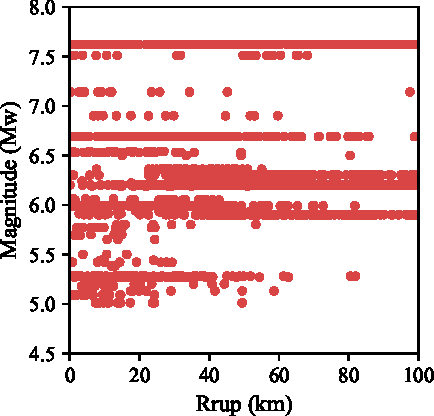
\includegraphics[width=0.45\textwidth]{Chapter-5/figs/GM_Selection.pdf}
	\caption{Mainshock selection from PEER NGA West2 database}
	\label{fig:GM_Selection}
\end{figure}

\begin{figure}[htbp]
	\centering
	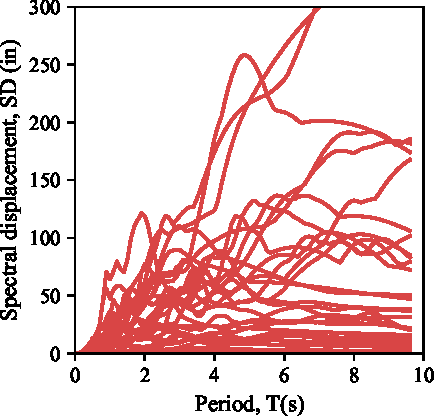
\includegraphics[width=0.45\textwidth]{Chapter-5/figs/SD_Spectrum_GM_Selection.pdf}
	\caption{Mainshock selection from PEER NGA West2 database}
	\label{fig:DisplacementSpectrum_Selection}
\end{figure}

\subsection{Modeling of mainshock-aftershock series for corrosion damage state}

Corrosion modifies the mechanical properties of rebars in RC structures, thus inherently modifying their response to earthquake loading. However, when an earthquake occurs is difficult to predict, as explained in section 2.4.2. Therefore, this study subjected structures with a specified corrosion level to a series of mainshock and aftershock ground motions. 
In order to analyze the structure to a sequence of mainshock and aftershock, it was necessary to glip together two ground motions. The process consisted of 1) selecting mainshocks and aftershocks from the same recording station and assigned to the same earthquake sequence, 2) the records were combined into a single file to run the sequence in order. The joined record also added a 4-second gap between the ground motions. This gap was to provide a sufficient amount of time for the record to reach stability. In contrast, the time to reach stability can vary depending on the structural and ground motion properties. A recommendation from Raghunandan et al. \cite{Raghunandan2015} found that 4s gives enough time for a structure to stabilize, a more significant time gap is possible, but it increases the computational cost significantly. An example of the resulting mainshock and aftershock sequence is shown in \fref{fig:MS-AS_sequence_sample}.

\begin{figure}[htbp]
	\centering
	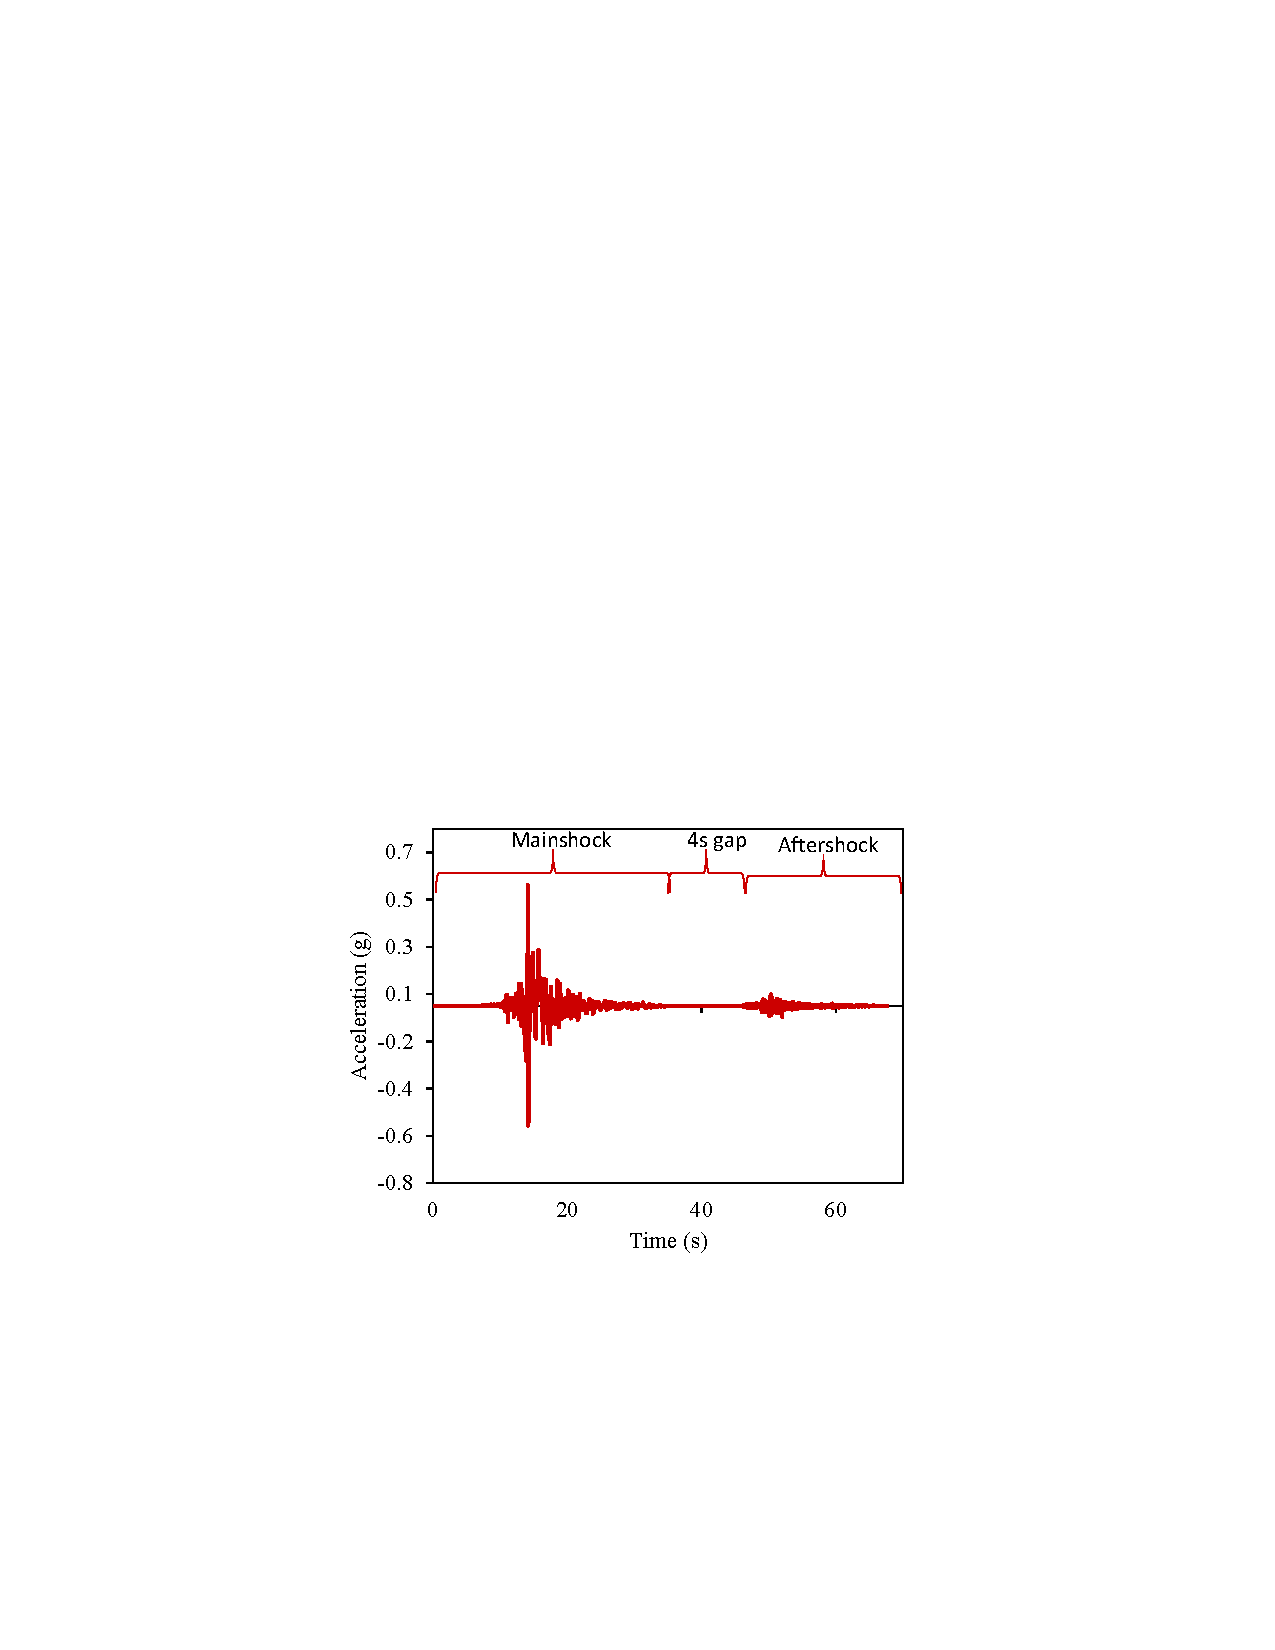
\includegraphics[width=0.6\textwidth]{Chapter-5/figs/MS_AS_Figure.pdf}
	\caption{Mainshock selection from PEER NGA West2 database}
	\label{fig:MS-AS_sequence_sample}
\end{figure}
\section{Analytical Model}
\subsection{Cantilever column}
This study focuses on the behavior of a single degree of freedom (SDOF) system representing a cantilever reinforced concrete column. The column is modeled as shown in \fref{fig:Structural_Model} This structure is modeled in OpenSeesPy \cite{McKenna2010}\cite{Zhu2018} using the $forceBeamColumn$ element \cite{Scott}. The forceBeamColumn element is used with two-point Gauss-Radau integration applied in the hinge regions and two-point Gauss integration applied on the element interior for a total of six integration points \cite{Scott}. The force-based formulation requires only a single element to accurately represent the full nonlinear deformation of the member and the integration scheme selected prevents the loss of objectivity during the softening response while also providing integration points at the member ends \cite{Calabrese2010},\cite{Scott}. The element requires the length of plasticity be defined at each end of the member, for which the tension-based rectangular plastic hinge length is calculated using the following expressions \cite{Goodnight2013}:

\begin{equation}
    L_{pc}=k*L_{eff} + 0.4D
    \label{eq:LP_Comp}
\end{equation}
\begin{equation}
	k=0.2*(Fu/Fy - 1) \leqslant 0.08
	\label{eq:K_Lp}
\end{equation}
\begin{equation}
    L_{pt}=L_{pc}+\gamma*D
    \label{eq:LP_Tension}
\end{equation}

For single bending the parameter $\gamma$ is:
\begin{equation}
    \gamma=0.33
    \label{eq:Gamma_LPt}
\end{equation}

The two-point Gauss-Radau integration is applied such that each end node integration is weighted equal to the specified plastic hinge length, as illustrated in \fref{fig:Fiber_PlasticHinge}. In this figure $D$ is the diameter of the column, and $c$ is the concrete cover. Therefore, strains recorded at the end sections represent accurate values even in the case where deformation localizes to the ends from strain-softening behavior. For the case of the cantilever column considered, only one plastic hinge length is defined, and the opposite end is given an arbitrary unit length. 

\begin{figure}[htbp]
	\centering
	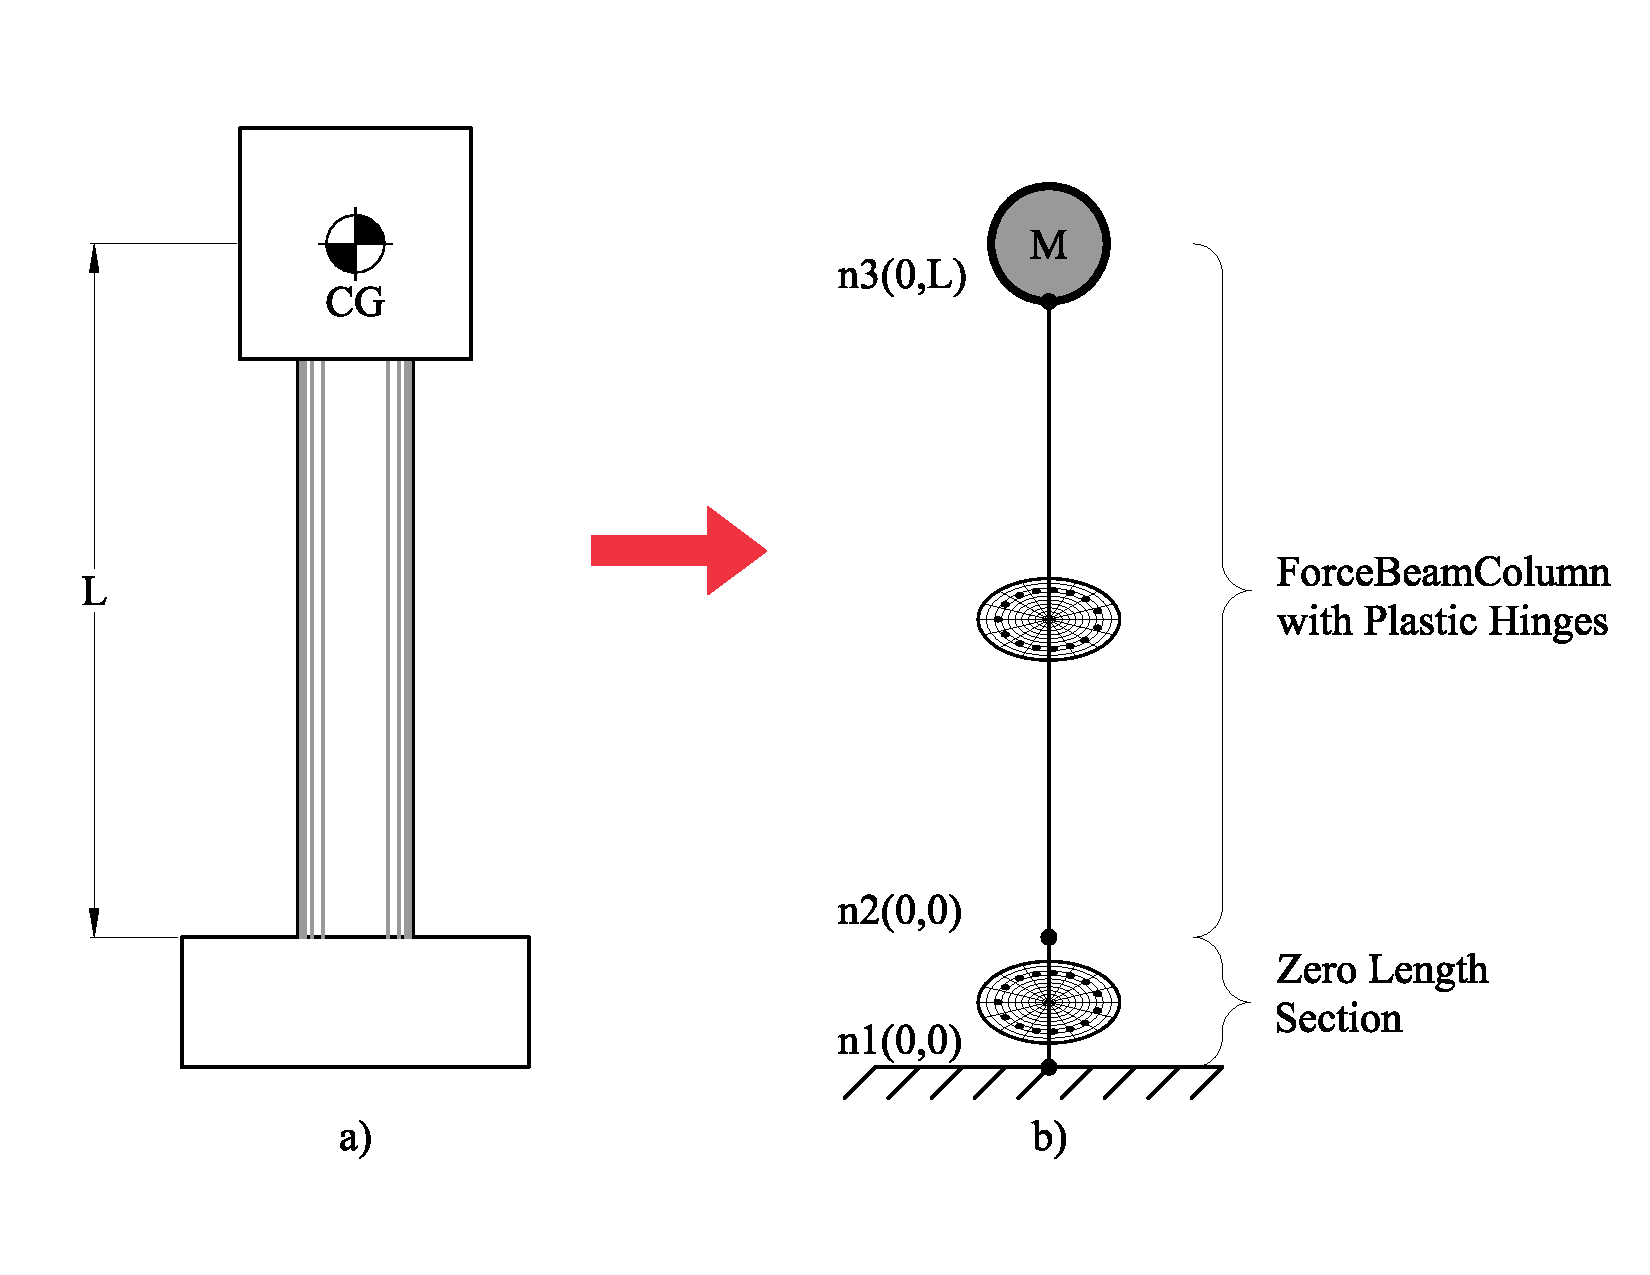
\includegraphics[width=0.75\textwidth]{Chapter-5/figs/StructuralModel_01}
	\caption{Structural Model a) SDOF Column b) Structural Model}
	\label{fig:Structural_Model}
\end{figure}

\begin{figure}[htbp]
	\centering
	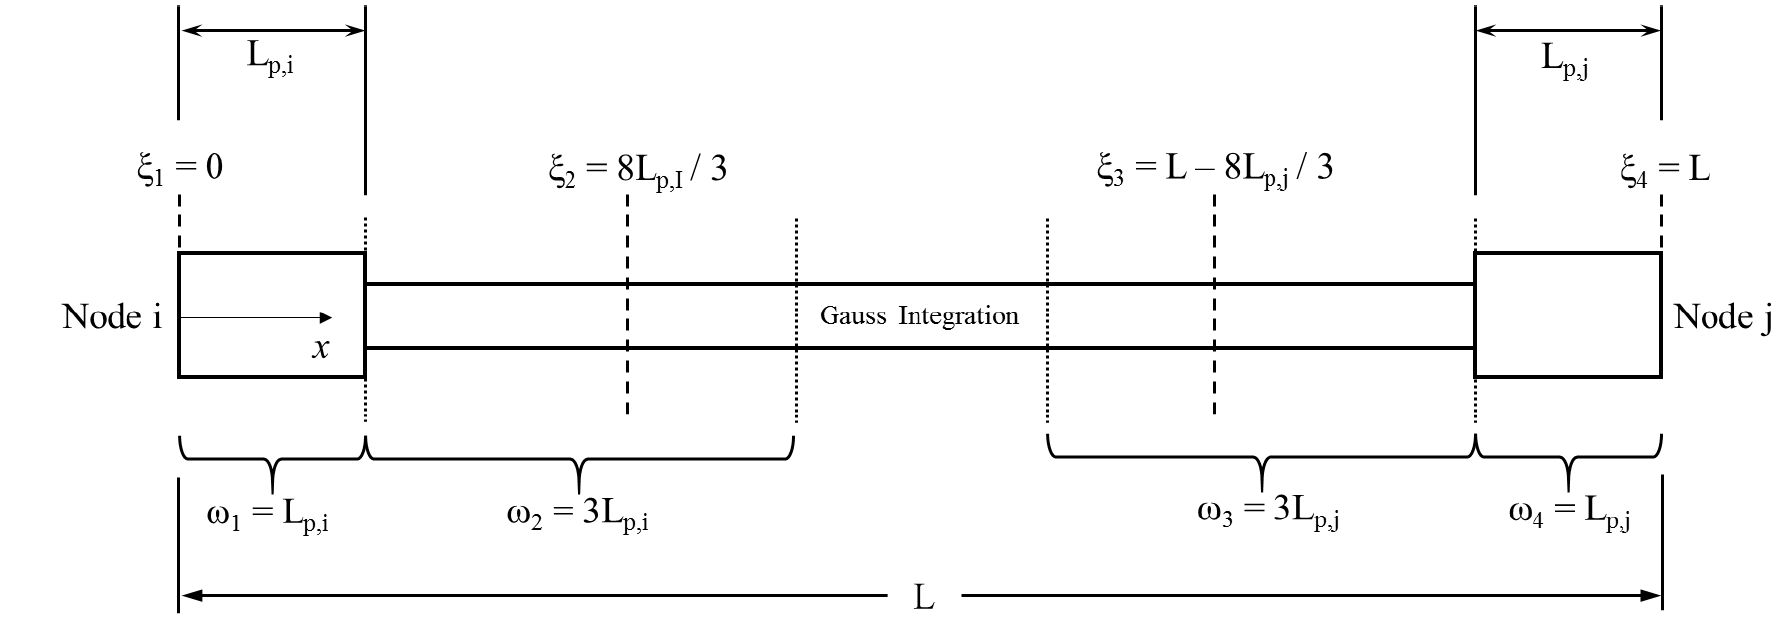
\includegraphics[width=0.9\textwidth]{Chapter-5/figs/fbc_PlasticHinge}
	\caption{End point plastic hinge method \cite{Scott}}
	\label{fig:Fiber_PlasticHinge}
\end{figure}

The cross section of the column is shown in \fref{fig:ColumnSection}. The column cross section is discretized with concrete and steel material fibers. Concrete fibers are modeled using the $Concrete01$ material, modified for confined material strength based on the Mander confined concrete model \cite{Mander1988}. The $Steel02$ material, based on the Giuffre-Menegotto-Pinto model \cite{Filippou1983} is used for the longitudinal reinforcement with recommended parameters ($b = 0.01, R0 = 20, cR1 = 0.925, cR2 = 0.15$). 

\begin{figure}[htbp]
	\centering
	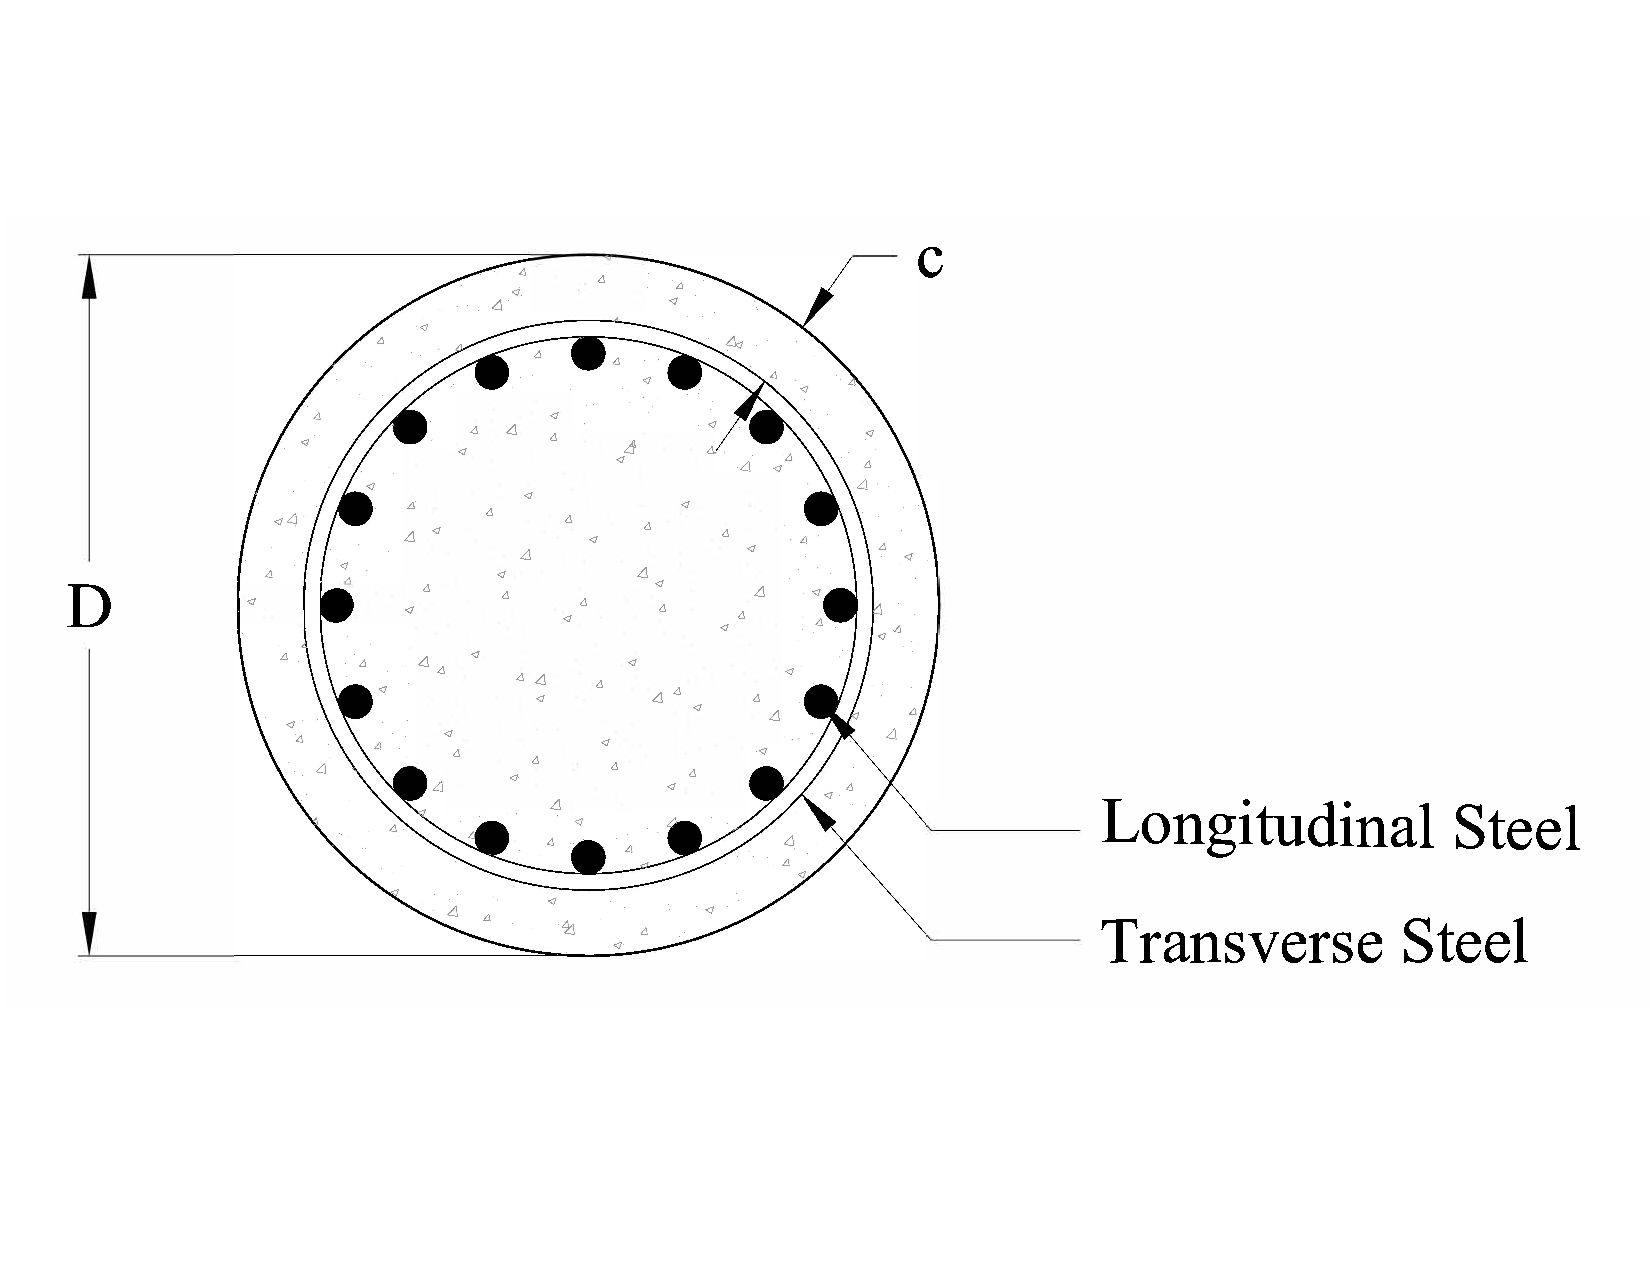
\includegraphics[width=0.7\textwidth]{Chapter-5/figs/StructuralModel_Section}
	\caption{Section of the RC Column}
	\label{fig:ColumnSection}
\end{figure}
\subsection{Strain penetration}

The strain penetration considers the additional deformation due to anchorage of the reinforcement into the foundation, since tension strain in the reinforcement will drop to zero at a depth equal to the true development length of the rebar \cite{Priestley2007}. Experimental studies have generally reported that this end rotation contributes up to 35\% to the lateral deformation of flexural members\cite{Zhao2007}. Therefore, it is important to incorporate it into the analytical model. A way to capture this effect is by using a zero-length section element implemented in the nonlinear fiber-based analysis of concrete structures, which is available in the material library of OpenSeesPy as $Bond SP1$ \cite{Zhao2007}. This is the material model used for the steel fibers of the zero-length section element.

The required parameters for this model are:
\begin{itemize}
	\item $F_{y}$ Yield strength of the reinforcement steel
	\item $S_{y}$ Rebar slip at member interface under yield stress (see \eref{eq.Rebar_Slip})
	\item $F_{u}$ Ultimate strength of the reinforcement steel
	\item $S_{u}$ Rebar slip at the loaded end at the bar fracture strength a value of $35 S_{y}$ is recommended \cite{Zhao2007}
	\item $b$ Initial hardening ratio in the monotonic slip vs. bar stress response $b=0.45$ is recommended \cite{Zhao2007}
	\item $R$ Pinching factor for the cyclic slip vs. bar response $R=1.01$ is recommended \cite{Zhao2007}
	\item $d_b$ Rebar diameter
	\item $f'c$ Concrete compressive strength of the adjoining connection member
	\item $\alpha$ Parameter used in the local bond-slip relation and can be taken as $\alpha=0.4$ in accordance with CEB-FIP Model Code 90 \cite{CEB1993}
\end{itemize}.
\newline
Bar slip is calculated as:
\begin{equation}
	S_{y}(in)=0.1\left(\frac{d_{b}F_{y}}{4000\sqrt{f'_{c}}}\left(2\alpha+1\right)\right)^{\frac{1}{\alpha}}+0.013 (in)
	\label{eq.Rebar_Slip}
\end{equation}
\subsection{Design limit states}
Design limit states are defined based on strains in the material since they can more accurately represent the different performance levels. Structure limit states are tension strains in the rebars or compression strains in the concrete core. The values recommended in the typical performance-based design of reinforced concrete bridge columns are shown in Table  \ref{tab:DesignLimitStates}. The serviceability limit states correspond to the compression strain at which concrete cover begins to crush and the peak tension strain, resulting in residual crack widths of approximately 1 mm. These limits are generally accepted as nominal limit states for RC members. The compression limit state for damage control is defined by the expression shown in Eq. \ref{eq:ec_DamageControl}, and it refers to the compression strain in the confined concrete at which fracture of the transverse reinforcement confining the core occurs \cite{Priestley2007}. This equation is obtained using the strain-energy balance between that absorbed by the confined core concrete and the capacity of the confining steel. The damage control limit state is defined by the strain at the onset of buckling, which can be expressed according to \ref{eq:es_DamageControl}. This model demonstrated accurate predictions of the onset of bar buckling on physical tests in SDOF Concrete Column \cite{Goodnight2016}. An additional limit state is the ultimate limit state, proposed by Barcley et al. \cite{Barcley2019}, which is defined as the previous tension strain before bar fracture due to bar buckling. The limit state can be expressed as shown in \eref{eq:es_ultimate}. For the case of corrosion, the effective material properties of the reinforcing steel bars are used, and in the case of the ultimate limit state, the equation that relates corrosion and the maximum bending strain is used.

\begin{equation}
    \varepsilon_{c,spiral yield}=0.009-0.3\frac{A_{st}}{A_{g}} +3.9\frac{f_{yhe}}{E_{s}}
    \label{eq:ec_DamageControl}
\end{equation}

\begin{equation}
    \varepsilon_{s,BB}=0.03+700\rho_{s}  \frac{f_{yhe}}{E_{s}} -0.1\frac{P}{f'_{c}A_{g}}
    \label{eq:es_DamageControl}
\end{equation}
\begin{equation}
    \varepsilon_{t}=\frac{ln(\frac{\varepsilon_{b}}{0.001})}{\frac{300P}{f'c A_{g}}+\frac{0.7}{\rho_{t}}}
    \label{eq:es_ultimate}
\end{equation}

\begin{table}[htpb]
	\caption{Design limit states}
	\label{tab:DesignLimitStates}
        \begin{center}
        \begin{tabular}{lll}
        Limit State         & Concrete Limit State (in/in) & Reinforcing Steel Limit State (in/in) \\ \hline
        Serviciability      & 0.04                         & 0.015                                 \\ 
        Collapse Prevention & \eref{eq:ec_DamageControl}   & \eref{eq:es_DamageControl}             \\ 
        Fracture            & N/A                          & \eref{eq:es_ultimate}                   \\ 
        \end{tabular}
        \end{center}
\end{table}

\section{Comparison with existing physical tests}
The model used in this research is calibrated for the case of pristine conditions and the case of corroded columns. The calibration to a pristine condition column shows how reliable the results from the model are. Then the pristine condition model is modified with the corrosion model, as explained in section 4.1.1. The analytical model is compared to the results from the physical test on corroded RC columns. This will give confidence that the results obtained from the analytical model are reliable, and will be further enhanced with the experimental results.
\subsection{Pristine condition columns}
Goodnight et al performed a total of 30 circular RC columns quasi-static tests to evaluate strain limit states \cite{Goodnight2016}. From this set of tests, a sample of one was taken to calibrate the analytical model. The test performed by Goodnight et al on an SDOF cantilever column shows similar geometry to that presented in \fref{fig:Fiber_PlasticHinge}. The parameters used in this large scale test were: diameter $D = 24.0 inch$, height of the column $L = 8.0 ft$, yield strength of steel $f_{y} = 574.0 MPa$, ultimate strength of steel $f_{u} = 753.3 * MPa$, longitudinal steel volumetric ratio $\rho_{s} = 1.5\% $, transverse steel volumetric ratio $\rho_{v} = 1.0\% $, and strength of concrete at 8 days $f'_{c} = 39.8 MPa$.

The analytical model used these parameters to compare the results from the model to the experimental results. The results from the analysis show good agreement with the experimental results as evidenced in \fref{fig:ModelCalibration}. Thus, the results obtained from the model predict the overall system behavior and can be used to analyze other configurations of the structural model.
\begin{figure}[htbp]
	\centering
	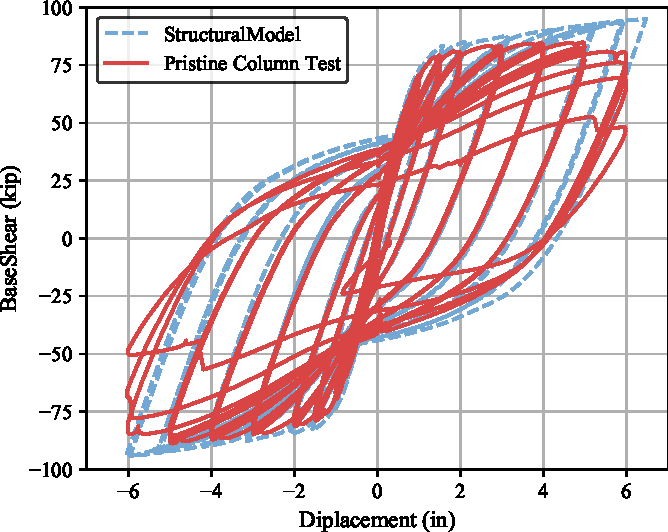
\includegraphics[width=0.60\textwidth]{Chapter-5/figs/Calibration_Test_26_Goodnight_et_al.pdf}
	\caption{Force-Displacement results from experimental results \cite{Goodnight2013} and analytical model}
	\label{fig:ModelCalibration}
\end{figure}

\begin{figure}[htbp]
	\centering
	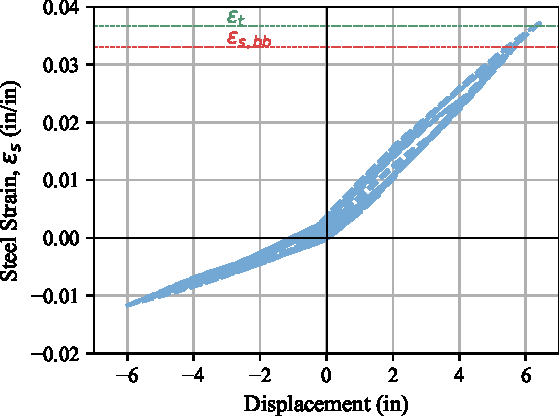
\includegraphics[width=0.5\textwidth]{VAC Thesis 2.0/Chapter-5/figs/Calibration_Test_26_Goodnight_et_al_strain.pdf}
	\caption{Strain hysteresis from experimental RC column in pristine condition}
	\label{fig:ModelCalibration_Pristine_Hysteresis}
\end{figure}

\subsection{Accelerated corrosion columns}
Similarly, Ma et al performed a series of quasi-static tests on RC columns with different corrosion levels and axial load ratios \cite{Ma2012}. From their study, the test with a corrosion level $CL=9.5\%$ was taken for calibration since the other tests presented in their study had excessively high axial load ratios which are not common in RC bridges. The results from Ma et al test	\cite{Ma2012} were used to compare against the analytical model. The column had the following parameters: diameter $D = 260.0 mm$, height of the column $L = 820.0 mm$, yield strength of steel $f_{y} = 375.0$ MPa, ultimate strength of steel $f_{u} = 572.3$ MPa, longitudinal steel volumetric ratio $\rho_{s} = 1.5\% $, transverse steel volumetric ratio $\rho_{v} = 1.0\% $, strength of concrete at 8 days $f'_{c} = 39.8$ MPa, and corrosion level $CL=9.5\%$. Equation \ref{eq.eleven} is used to modify the material properties of the reinforcing steel and considers the effects of corrosion. 

\begin{figure}[htbp]
	\centering
	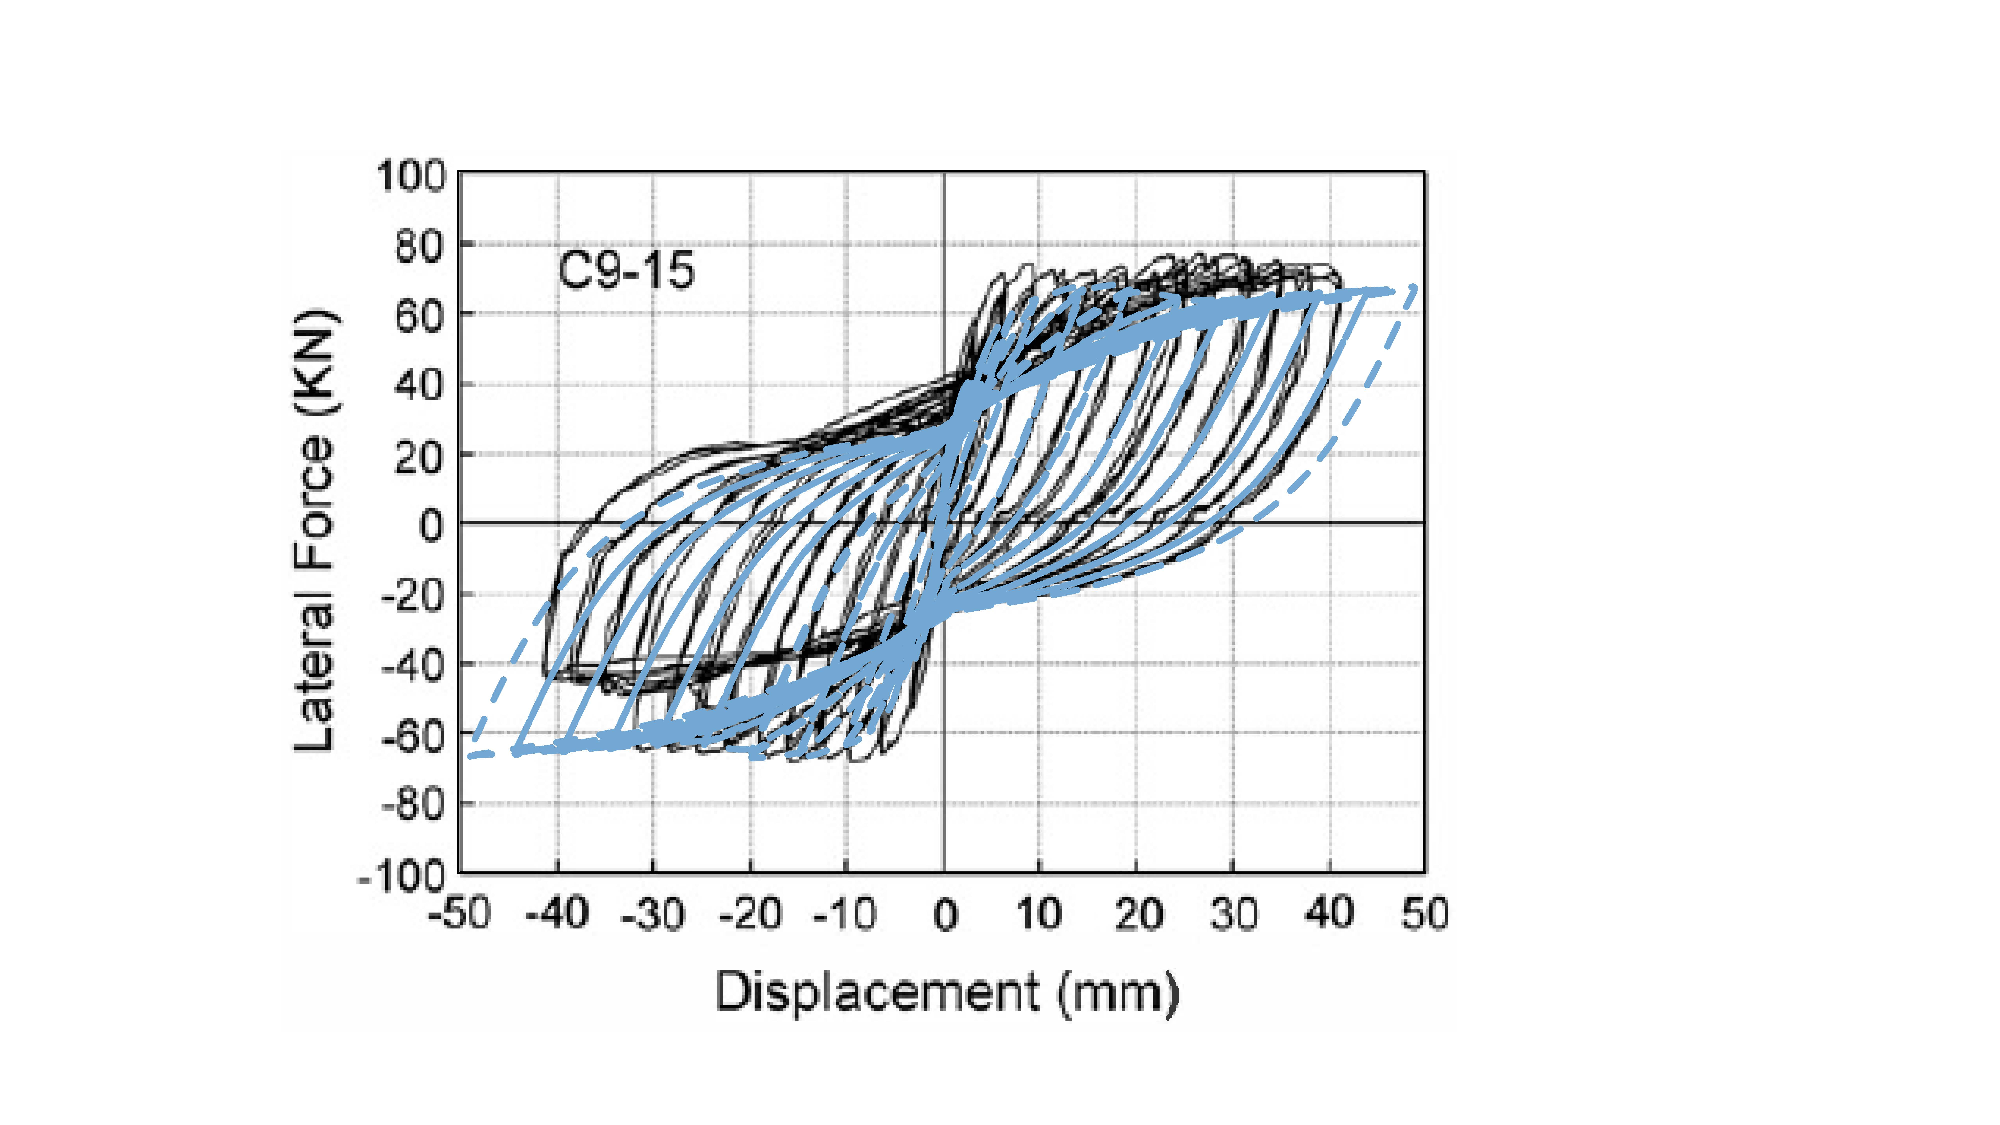
\includegraphics[width=0.50\textwidth]{Chapter-5/figs/Model_vs_MaEtAl_220218.pdf}
	\caption{Force-Displacement results from experimental RC column with corrosion in logitudinal bar (CL=9.5\%) \cite{Ma2012} and analytical model results (shown in lightblue)}
	\label{fig:ModelCalibration_Corrosion}
\end{figure}

Figure \ref{fig:ModelCalibration_Corrosion} shows that the results obtained from the analytical model capture the response of the structure with good accuracy. Ma et al \cite{Ma2012} did not report if bar buckling and bar fracture occurred during the test. However, the hysteresis curve shown in their study suggests that some damage limit state was reached. Therefore, \eref{eq:es_DamageControl} is used to determine the bar buckling limit state ($\varepsilon_{s,BB}=0.024$), this is then compared to the analytical model results shown \fref{fig:ModelCalibration_Corrosion_Hysteresis}. The results show a peak tension strain of $\varepsilon_{s}=0.023$, which is close to the value obtained using equation \eref{eq:es_DamageControl}. Therefore, there is a high likelihood that the bar buckling limit state was reached during this test. While these results are close, it is still not clear if \eref{eq:es_DamageControl} captures the behavior of the buckling limit state for corroded rebars. Thus, the proposed corroded BBT test will show if corrosion affects the behavior of buckled bars.

\begin{figure}[htbp]
	\centering
	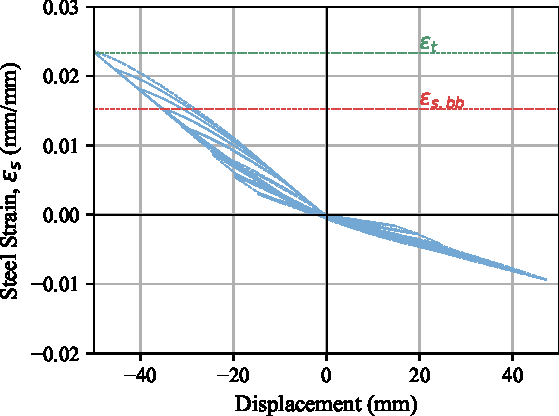
\includegraphics[width=0.5\textwidth]{VAC Thesis 2.0/Chapter-5/figs/Calibration_Ma_et_al_strain.pdf}
	\caption{Strain hysteresis from experimental RC column with corrosion in longitudinal bar (CL=9.5\%) results from analytical model}
	\label{fig:ModelCalibration_Corrosion_Hysteresis}
\end{figure}
\newpage
\section{Intensity Measure: $Sd(T_{eff},\xi)$}

When relating ground motions to structural response parameters, selecting appropriate quantities that accurately capture their relationship is crucial. Krish \cite{Krish2018} showed in a recent study that there is a good correlation between strain obtained from fiber modeling and first mode effective spectral displacement ($IM=Sd(T_1)$). On the other hand, peak ground acceleration $(PGA)$ did not correlate well. These conclusions are congruent with the results found by Mackie et al. \cite{Mackie2003}. 

In this study, the intensity measure was improved further by correlating the strains to the effective period of the structure $(T_{eff}$ and the equivalent damping $(\xi)$. These parameters are of substantial use in the Direct Displacement Based Design Methodology. The calculation of the effective period of the structure and the equivalent damping are explained below.

\subsection{Effective period calculation}

The process to calculate the effective period consists in obtaining first the effective stiffness of the structure. From the Non-Linear Time History Analysis (NLTHA) of a structure, the maximum displacement and force at the maximum displacement are obtained, as shown in \fref{fig:k_eff_calc}. With these values, the effective stiffness can be calculated as:

\begin{equation}
     K_{eff}=\frac{F(d_{max}}{d_{max}}
    \label{eq:Keff_calcualtion}
\end{equation}

\begin{figure}[htbp]
	\centering
	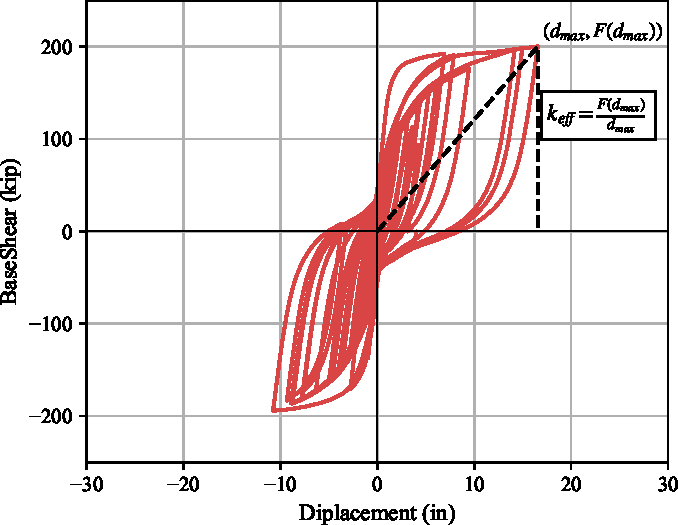
\includegraphics[width=0.60\textwidth]{VAC Thesis 2.0/Chapter-5/figs/Force_Diplacement_Keff_Calc.pdf}
	\caption{Calculation of effective stiffness $(k_{eff})$}
	\label{fig:k_eff_calculation}
\end{figure}

After obtaining the effective stiffness, the effective period can be calculated with the relationship for the period of a structure. The effective period is calculated as:

\begin{equation}
     T_{eff}=2\pi \sqrt{\frac{M}{K_{eff}}}
     
    \label{eq:Teff_calcualtion}
\end{equation}

In the analytical program the mass is calculated on the basis of the axial load applied to the structures. 

\begin{equation}
    M=\frac{P}{g}
    \label{eq:M_calcualtion}
\end{equation}

\subsection{Calculate $Sd(T_{eff},\xi)$}

After obtaining the effective period for each ground motion, it is possible to obtain the spectral displacement at 5\% damping for each ground motion for a given effective period. Finally, the equivalent damping that the system reached for a given ground motion must be found to obtain the spectral displacement at the effective period and equivalent damping. Using the expressions for equivalent damping from Priestley et al. for circular columns in bridges, the equivalent damping can be expressed as:

\begin{equation}
    \xi_{eq}=0.05+0.444\frac{\mu-1}{\mu\pi}
    \label{eq:EqDamping_calcualtion}
\end{equation}

The damping factor that corresponds to the equivalent damping is calculated as:

\begin{equation}
    DF=\sqrt{\frac{0.07}{0.02+\xi_{eq}}
    \label{eq:DF_calcualtion}
\end{equation}

Equations \eref{eq:EqDamping_calcualtion} and \eref{eq:DF_calcualtion} are part of the DDBD procedure outlined by Priestley et al \cite{Priestley2007}. Finally, the spectral displacement at effective period and equivalent damping can be expressed as:


\begin{equation}
    Sd(T_{eff},\xi)=DF Sd(T_{eff},5\%)
\end{equation}

The preceeding methodology can be seen graphically in \fref{fig:SpectralDisplacementCalculation}

\begin{figure}[htbp]
	\centering
	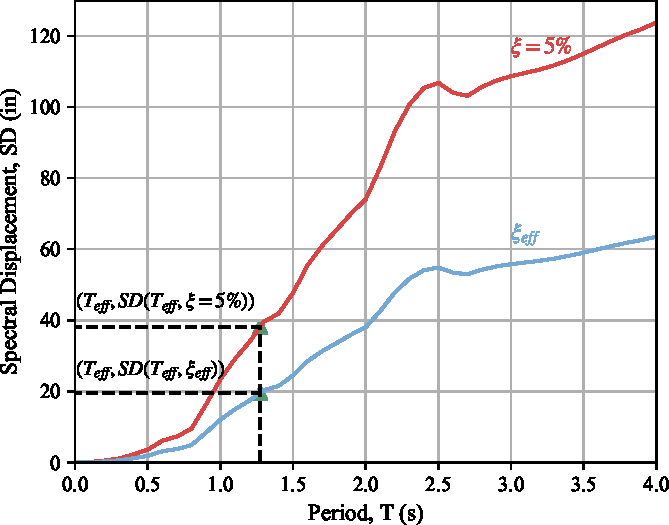
\includegraphics[width=0.6\textwidth]{VAC Thesis 2.0/Chapter-5/figs/SpectralDisplacement_SD(Teff,xi)_Calc.pdf}
	\caption{Calculation of spectral displacement at effective period at 5\% damping $Sd(T_{eff},5\%)$ and at equivalent damping $Sd(T_{eff},\xi)$}
	\label{fig:SpectralDisplacementCalculation}
\end{figure}

\section{Anlsysis of results using MSA}

Once the analysis is complete the data is post-processed and expressed as a cumulative distribution function (CDF). The methodology employed corresponds to the multiple stripe analysis (MSA) recommended by Baker et al \cite{Baker2015}. While peak ground acceleration ($PGA$) has been widely used as the intensity measure to develop fragility functions\cite{Ghosh2015}\cite{Bisadi2015}\cite{Shekhar2018}. Krish \cite{Krish2018} showed in a recent study, that spectral displacement at first effective period ($IM=Sd(T_1)$) has better correlation than $PGA$. To demonstrate this, CDF curves were developed for $IM=PGA$ and $IM=Sd(T_1)$, and are shown in \fref{fig:CDF_SY_PGA} and \fref{fig:CDF_SY_SDT1} respectively. The CDFs were developed for the steel yielding limit state; however this can be the extrapolated for any limit state. \fref{fig:CDF_SY_PGA} shows the results obtained with $IM=PGA$ do not show a good correlation since as corrosion increases the probability of exceeding a limit state decreases. This is not the behavior observed in \fref{fig:Steel_Stress_Strain_Response}. Conversely, \fref{fig:CDF_SY_SDT1} shows the results with $IM=Sd(T_1)$. These results present a better correlation, since, as corrosion increases, the probability of exceeding the limit state of yielding increases. For the preliminary results shown here, the corrosion level of 13.1\% results are an exception. These results will improve as more analyses become available. 

\begin{figure}[htp]
	\centering
	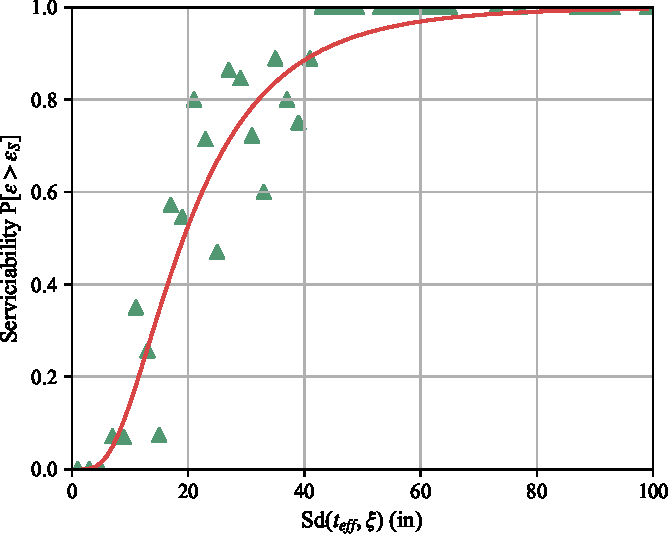
\includegraphics[width=0.60\textwidth]{VAC Thesis 2.0/Chapter-5/figs/MSA_Calc.pdf}
	\caption{MSA analysis}
	\label{fig:msa_sample_01}
\end{figure}

\section{Analytical framework}

The analytical framework was established to obtain the change in the structure performance due to aging conditions and to evaluate the effect of seismic events on the strain performance of single degree of freedom columns. This framework consisted of a program that performed and analyzed a series of nonlinear time history analyses (NLTHA). From these analyses, it was then possible to determine the effects of damage in the performance of structures. The proposed analytical framework process consisted of:

\begin{enumerate}
	\item Geometrical properties of the SDOF column 
	\item The effective mechanical properties of the reinforcing steel were evaluated.
	\item Nonlinear time history analyses of discrete ground motions and sequence of ground motions
	\item Posprocessing of data
\end{enumerate}

The analysis matrix for the corrosion aging phenomenon that was analyzed in this study is shown in Table \ref{tab:AnalysisMatrix}. The area or extent covered in the analysis corresponds to the range of variables that are common for RC columns in bridges.These analysis matrix resulted in a total of 36,000 analysis for the discrete ground motion analysis and 96,000 analysis for the sequences of ground motion case. To perform this large volume of analysis the Henry2 High Performance Computer (HPC) was used, to run the analysis in parallel. 

\begin{table}[htb]
	\caption{Analysis matrix}
	\label{tab:AnalysisMatrix}
	\centering
\begin{tabular}{{lcc}}
Parameter                          & Parameter        & Range                  \\	\hline
Diameter of column                     & D                & 28-90 in               \\	
Column aspect ratio        & L/D              & 4-8                    \\	
Longitudinal ratio                     & $\rho_s$         & 0.01-0.04              \\	
Axial load ratio                       & ALR              & 5\%-20\%               \\	
Corrosion level                         & CL               & 0\%-20\%               \\	
\end{tabular}
\end{table}

\subsection{Analysis Algorithm}

In order to run the analysis efficiently, a program was developed to perform three main routines:
1) Main program: setting conditions, the geometry of the model, effective material properties, 2) Run the Non-Linear Time History Analysis, 3)Post-processing of data

The main program is shown in \fref{fig:main_flowchart}. This program has three main inputs the ground motion records, the geometry of the column, and the aging conditions, which correspond to the corrosion level, the initial material properties, the axial load ratio, and the aspect ratio. After the inputs are done, a nested loop that goes through the different parameters is performed. The basic flow consists of preparing the data into the NLTHA subroutine and the post-processor subroutine. Once the program goes through the subroutines, the data output from OpenSees is deleted to use the HPC resources efficiently. This process is repeated until all the variables have been evaluated and the program finishes.

\begin{figure}[htp]
	\centering
	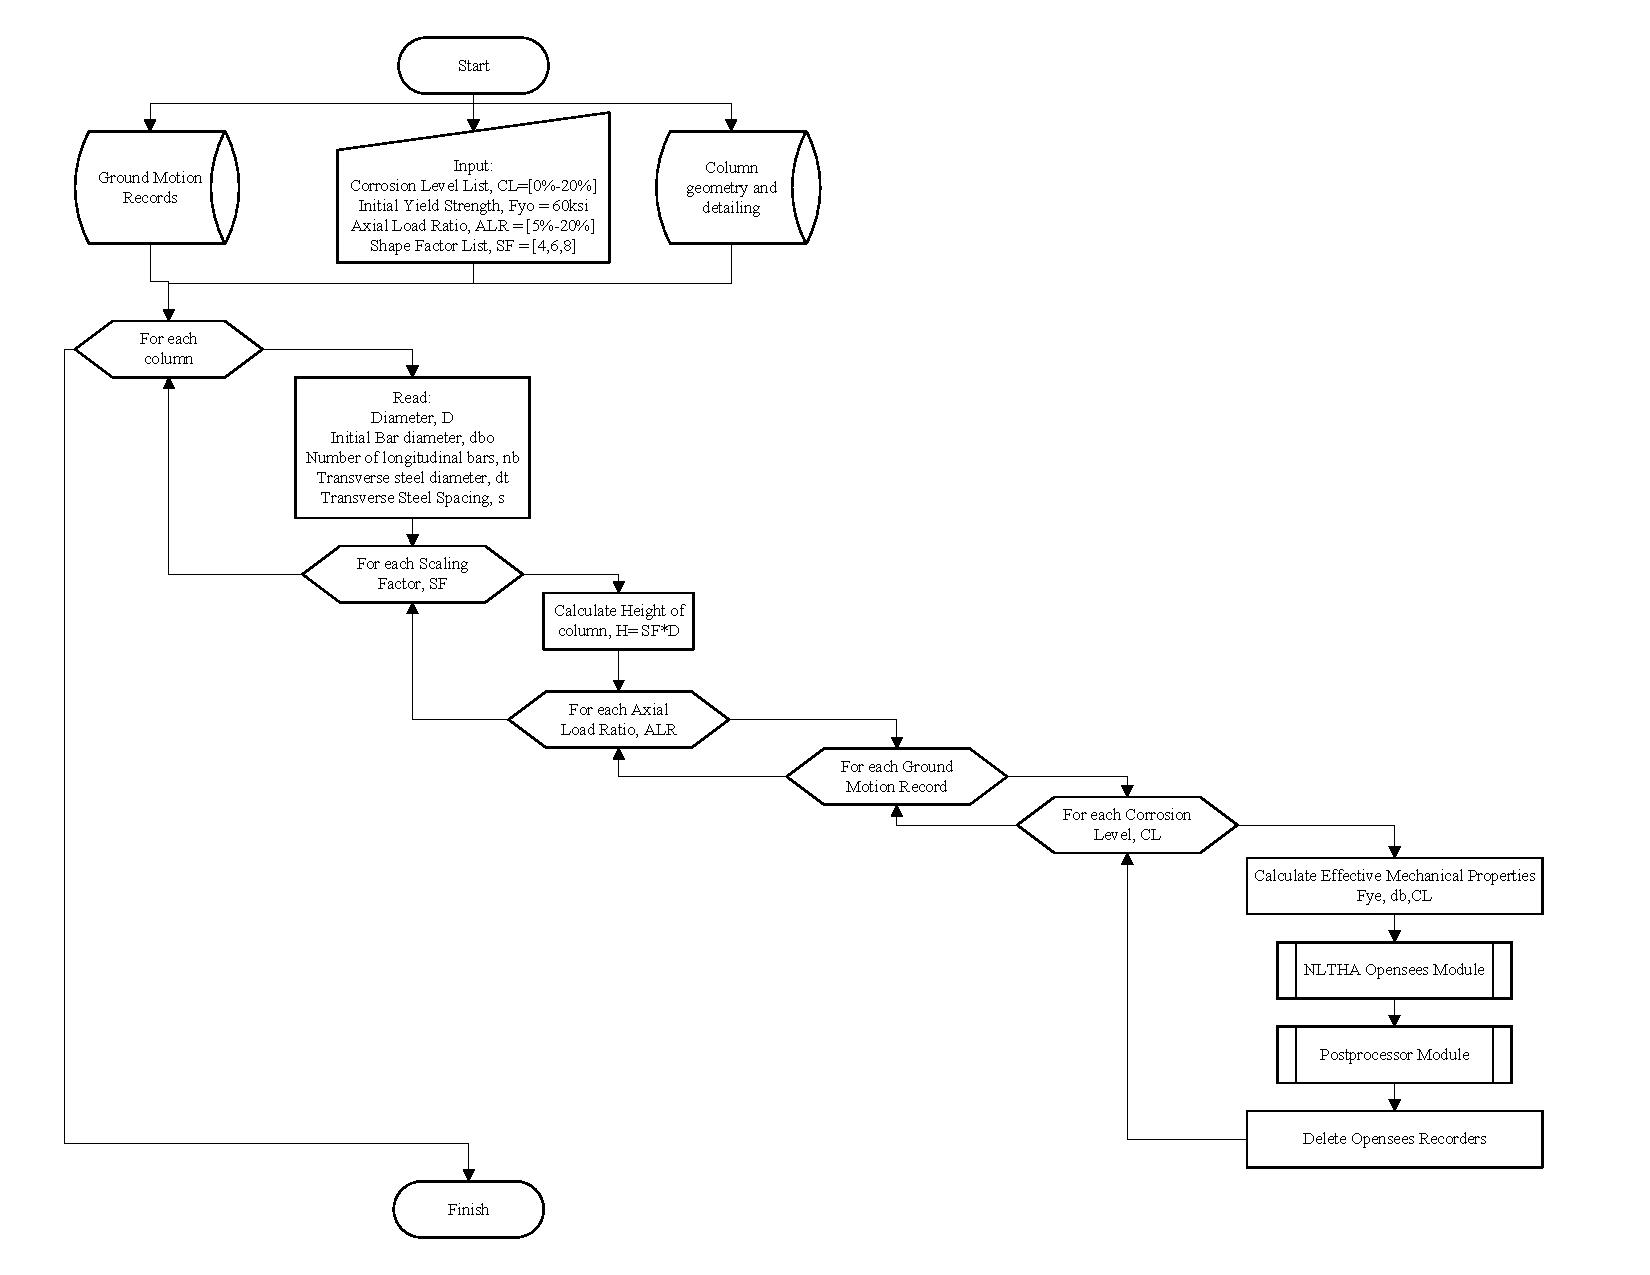
\includegraphics[width=0.975\textwidth]{VAC Thesis 2.0/Chapter-5/figs/Main_FlowChart_01.pdf}
	\caption{Main Flow-Chart}
	\label{fig:main_flowchart}
\end{figure}

The NLTHA subroutine consisted of a sequential process as shown in \fref{fig:nltha_flowchart}. First, the geometry of the model is established as per the model shown in \fref{fig:Structural_Model}. Then the material properties and the cross-sectional fibers are defined. Next, the recorders that store the analysis results throughout the NTLHA are set. Then the axial load is run and kept constant through the analysis. Finally, the NLTHA is run until it finishes.

\begin{figure}[htp]
	\centering
	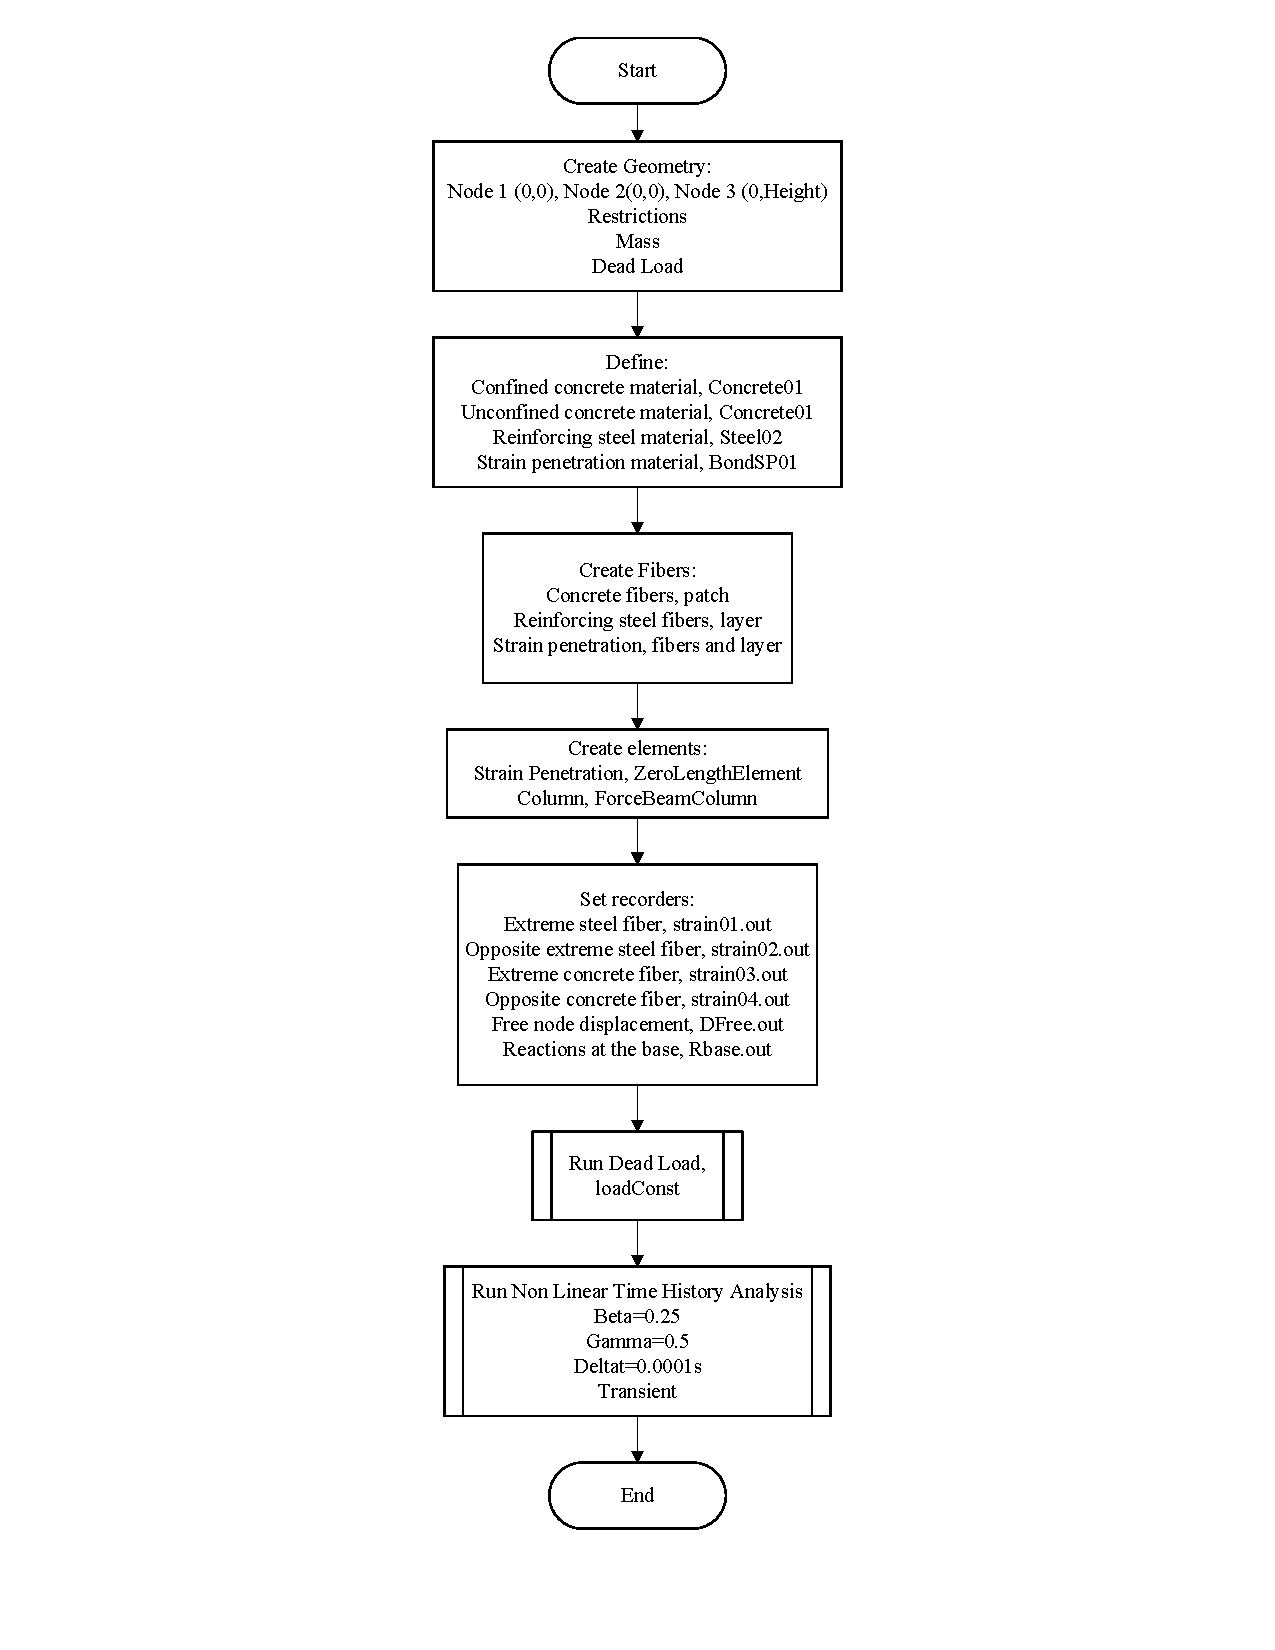
\includegraphics[width=0.425\textwidth]{VAC Thesis 2.0/Chapter-5/figs/NLTHA_FlowCharts_01.pdf}
	\caption{NLTHA Flow-Chart}
	\label{fig:nltha_flowchart}
\end{figure}

The post-processor subroutine also consisted of a sequential process as shown in \fref{fig:postproc_flowchart_01} and \fref{fig:postproc_flowchart_02} . The main goal of this subroutine is to store the data related to the model, including the geometry and material properties used in the analysis. The post-processor calculates the limit states as explained in section 5.3.3. Then the spectral displacement at the effective period is calculated for the ground motion following the procedure explained in section X.X. Finally, a collapse analysis for each limit state is performed in order to perform the multi-stripe analysis explained in the following section, all the relevant data is then stored in a database for further analysis.

\begin{figure}[htp]
	\centering
	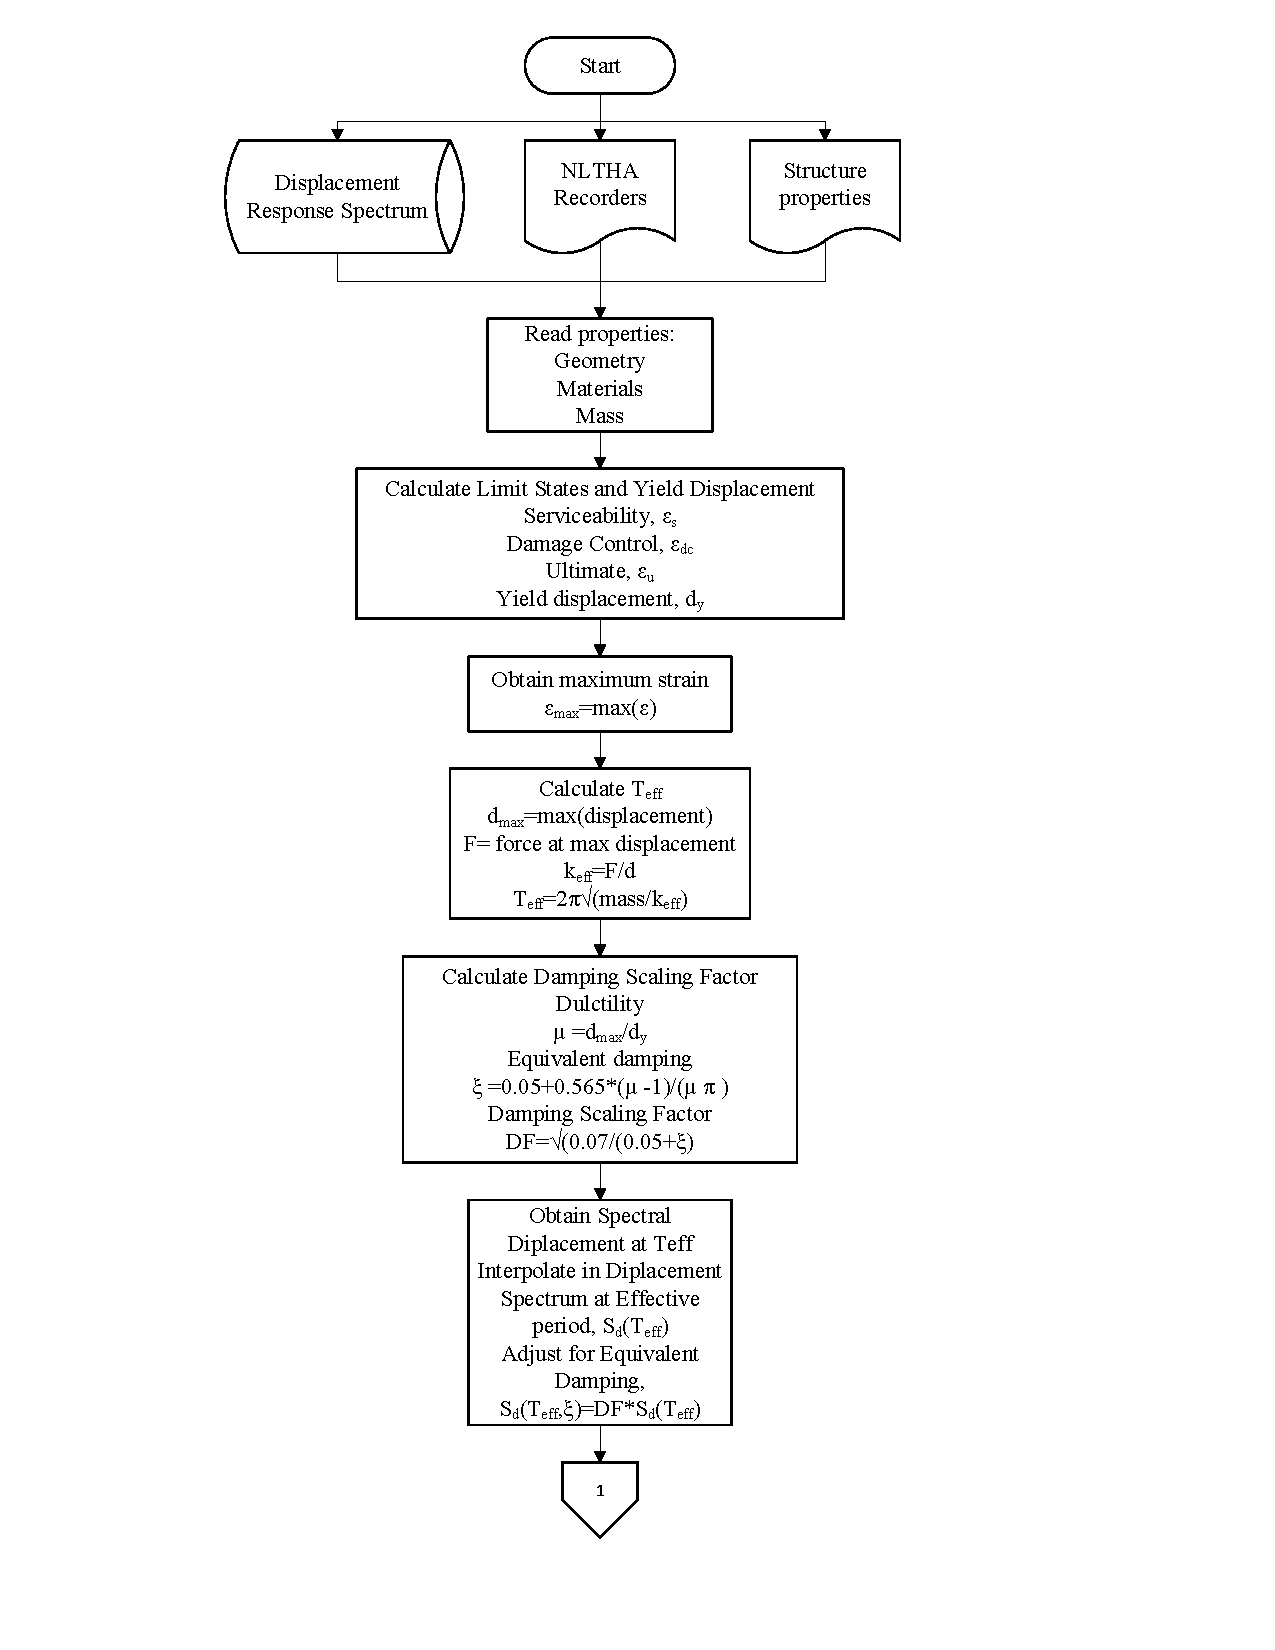
\includegraphics[width=0.575\textwidth]{VAC Thesis 2.0/Chapter-5/figs/PostProcessor_FlowCharts_01.pdf}
	\caption{Post-processor Flow-Chart}
	\label{fig:postproc_flowchart_01}
\end{figure}

\begin{figure}[htp]
	\centering
	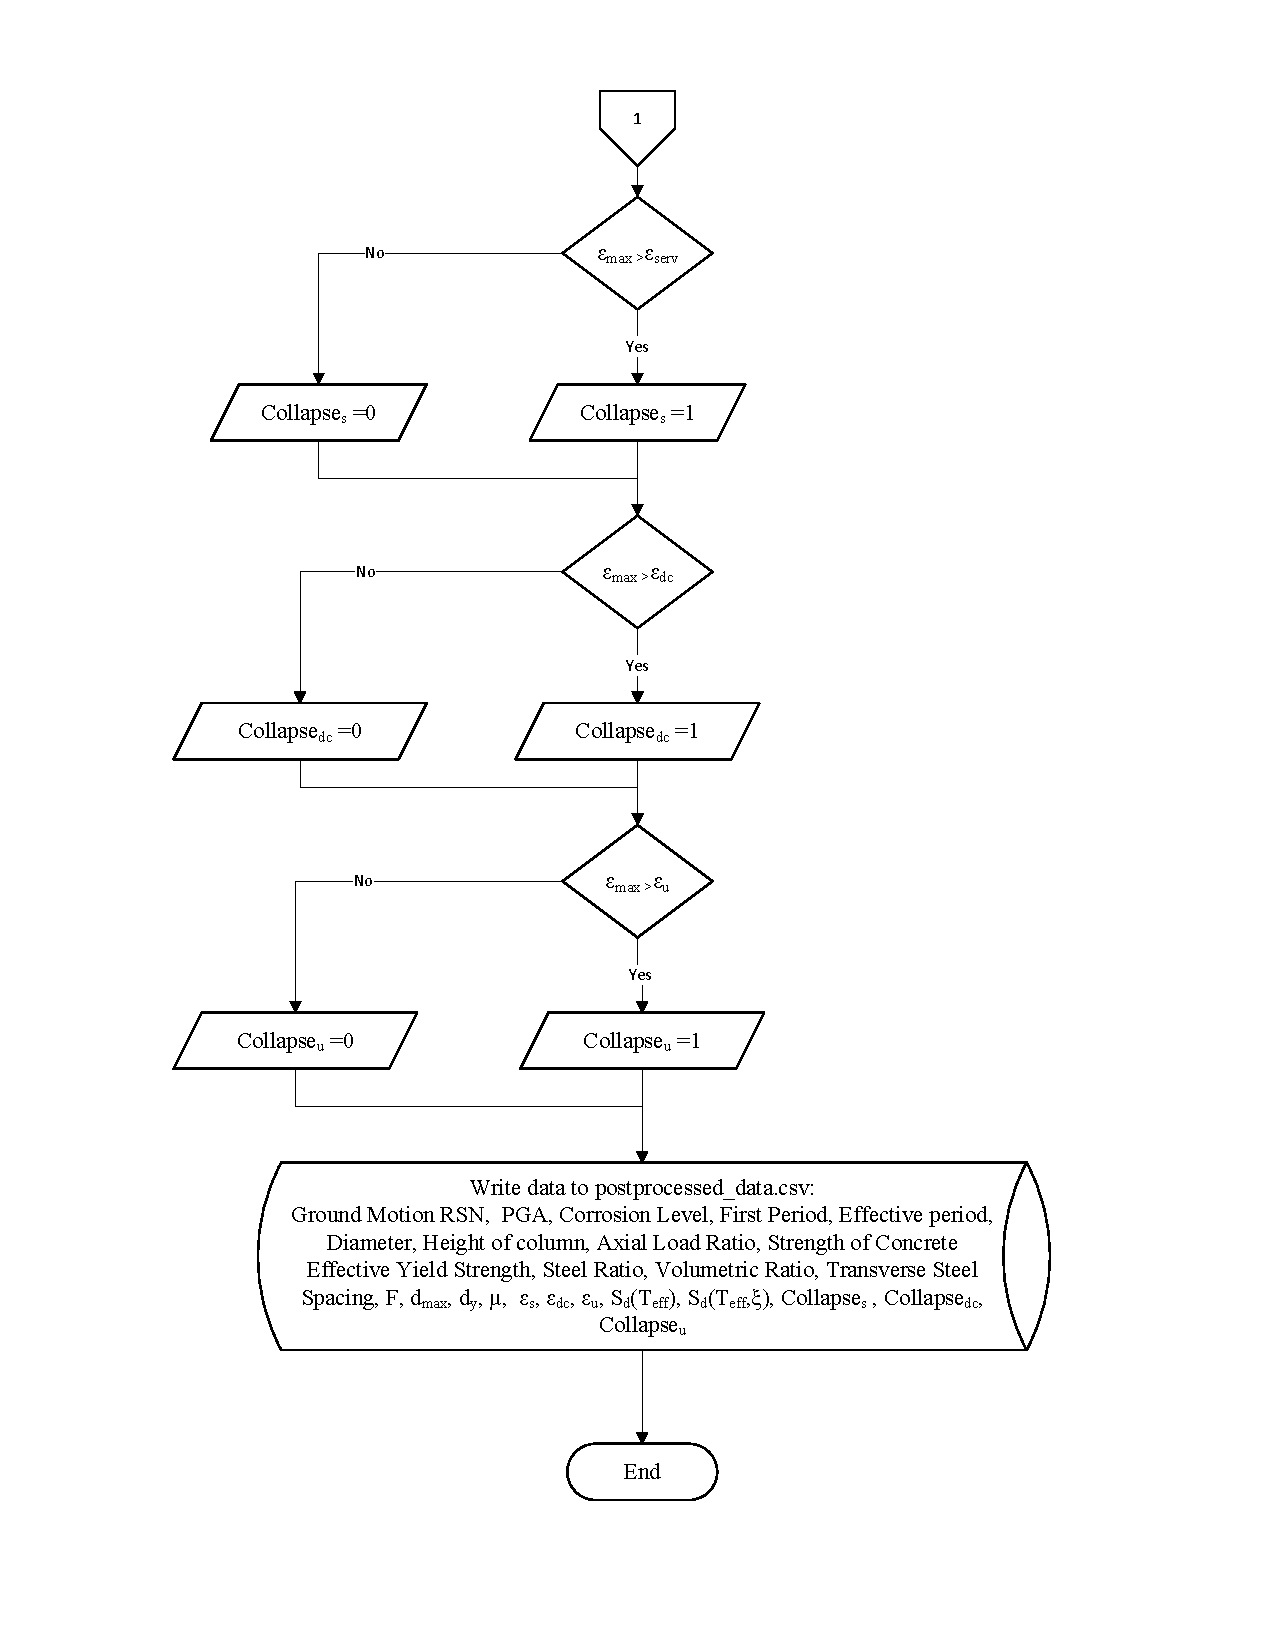
\includegraphics[width=0.75\textwidth]{VAC Thesis 2.0/Chapter-5/figs/PostProcessor_FlowCharts_02.pdf}
	\caption{Post-processor Flow-Chart continued}
	\label{fig:postproc_flowchart_02}
\end{figure}




%This procedure has been summarized in the form of a flow chart presented in \fref{fig:NLTHA_Framework}
%
%\begin{figure}[htbp]
%	\centering
%	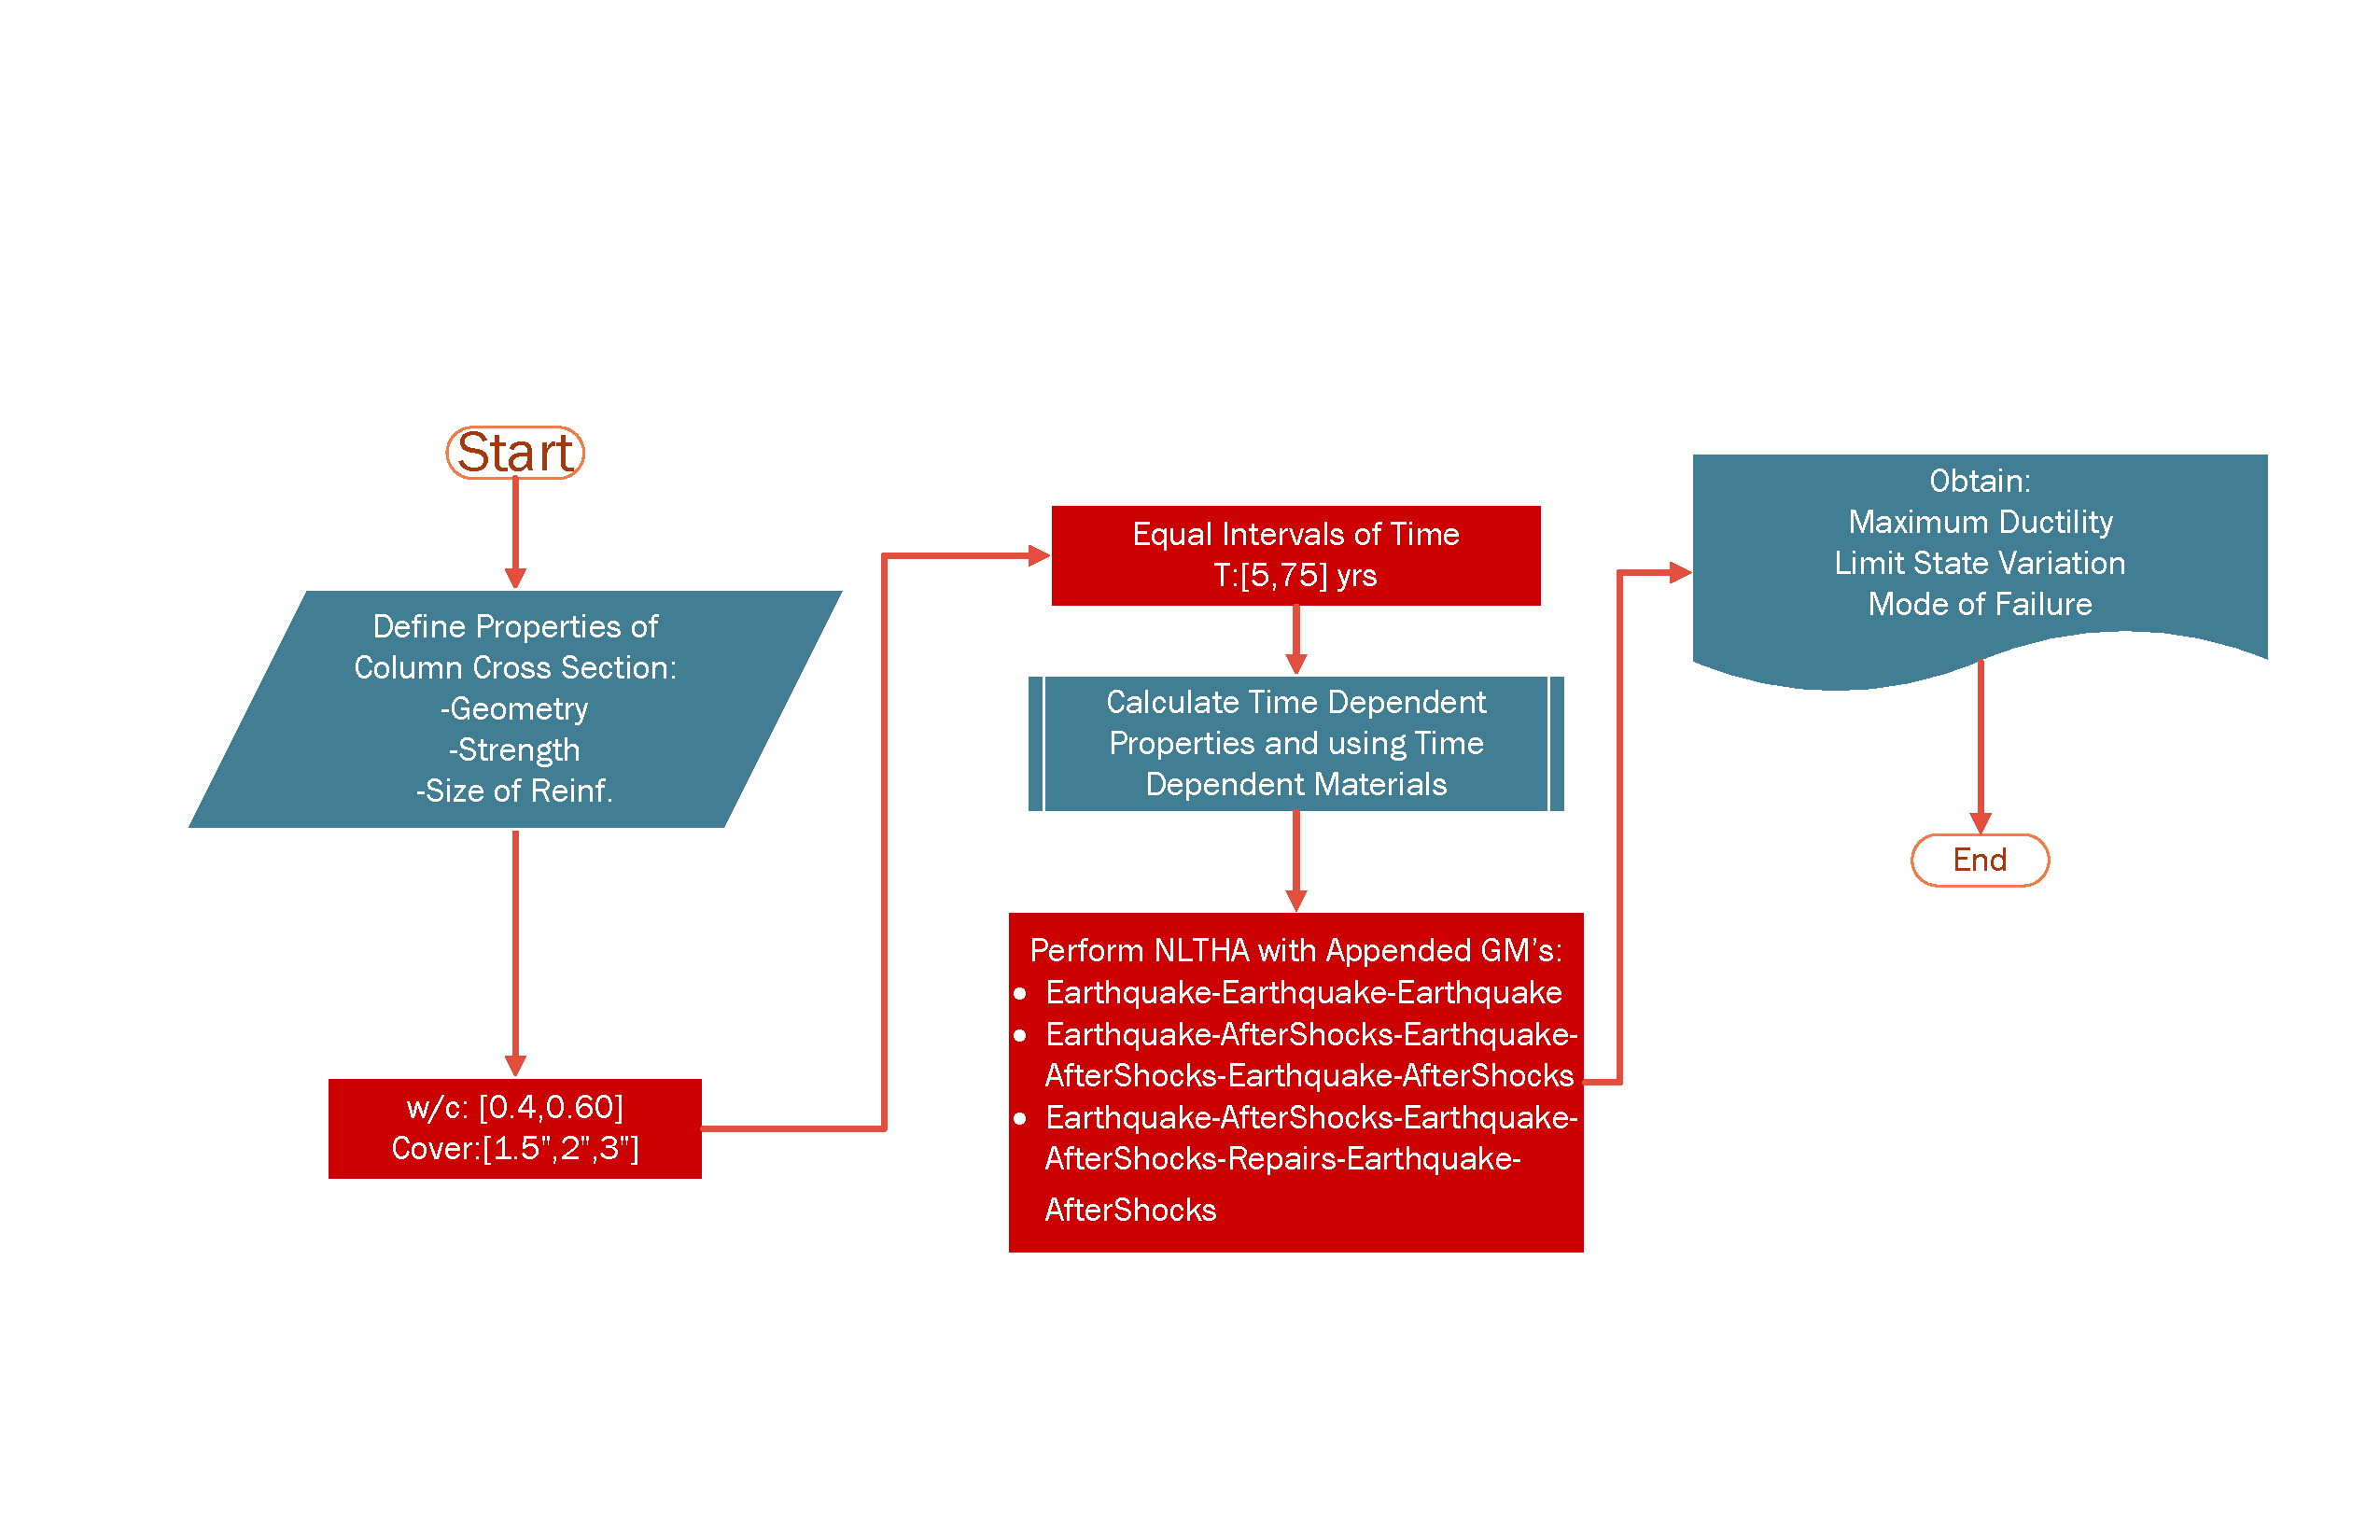
\includegraphics[width=0.9\textwidth]{Chapter-5/figs/AnalysisFramework_01}
%	\caption{Analysis Framework Flowchart}
%	\label{fig:NLTHA_Framework}
%\end{figure}
%
%\section{Earthquake selection}
%\lipsum[4]
\section{Results from Analytical Program}
This section presents the results obtained from a non-linear time history analysis (NLTHA) performed using OpenSeesPy \cite{Zhu2018}. The structure was subjected to a total of 18 earthquake records. The primary responses obtained from these analyses correspond to the maximum strain obtained for the different levels of corrosion. The structure was analyzed for a range of corrosion levels [1.5\%-13\%] in the longitudinal rebars.

\subsection{Structural Response at Different Corrosion Levels}
Figures \ref{fig:Force-Displacement_Results} and \fref{fig:Steel_Stress_Strain_Response} are presented as an example of the results obtained using NLTHA. These results are extracted from the structure's response to the Chi-Chi earthquake. \fref{fig:Force-Displacement_Results} shows the global system response and \fref{fig:Steel_Stress_Strain_Response} shows the stress-strain response of the extreme fiber of reinforcing steel. These results show that as corrosion increases, the demands imposed on the structure increase too. Therefore, the probability of reaching a limit state increases as corrosion increases.

\begin{figure}[htbp]
	\centering
	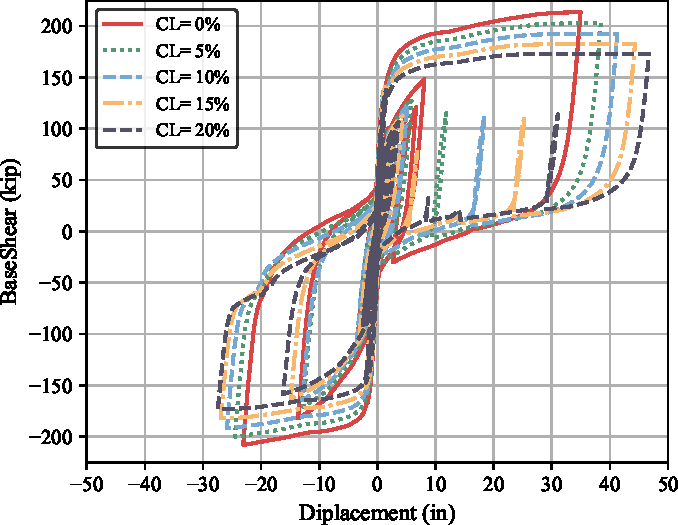
\includegraphics[width=0.7\textwidth]{Chapter-5/figs/Force_Diplacement_RSN1505.pdf}
	\caption{Force-Displacement results}
	\label{fig:Force-Displacement_Results}
\end{figure}

\begin{figure}[htbp]
	\centering
	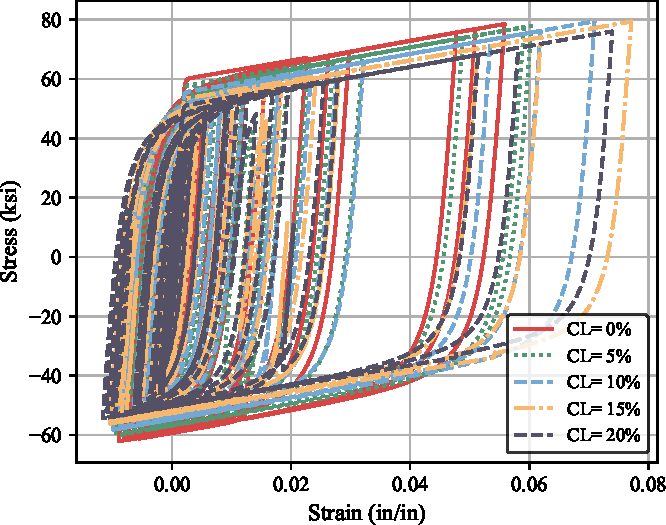
\includegraphics[width=0.7\textwidth]{Chapter-5/figs/Stress_Strain_RSN1505.pdf}
	\caption{Stress strain response for extreme rebar location}
	\label{fig:Steel_Stress_Strain_Response}
\end{figure}

\begin{figure}[htbp]
	\centering
	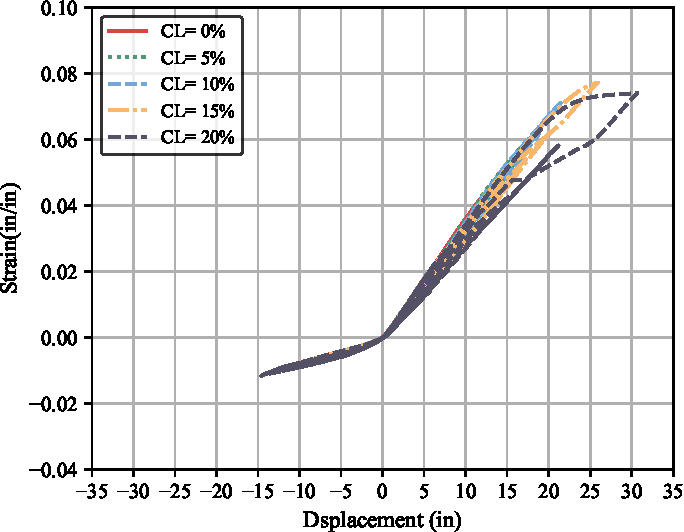
\includegraphics[width=0.7\textwidth]{Chapter-5/figs/Diplacement_Strain_RSN1505.pdf}
	\caption{Strain hysteresis}
	\label{fig:Steel_Stress_Strain_Response}
\end{figure}

\subsection{Effect of groundmotion sequences}

\begin{figure}[htbp]
	\centering
	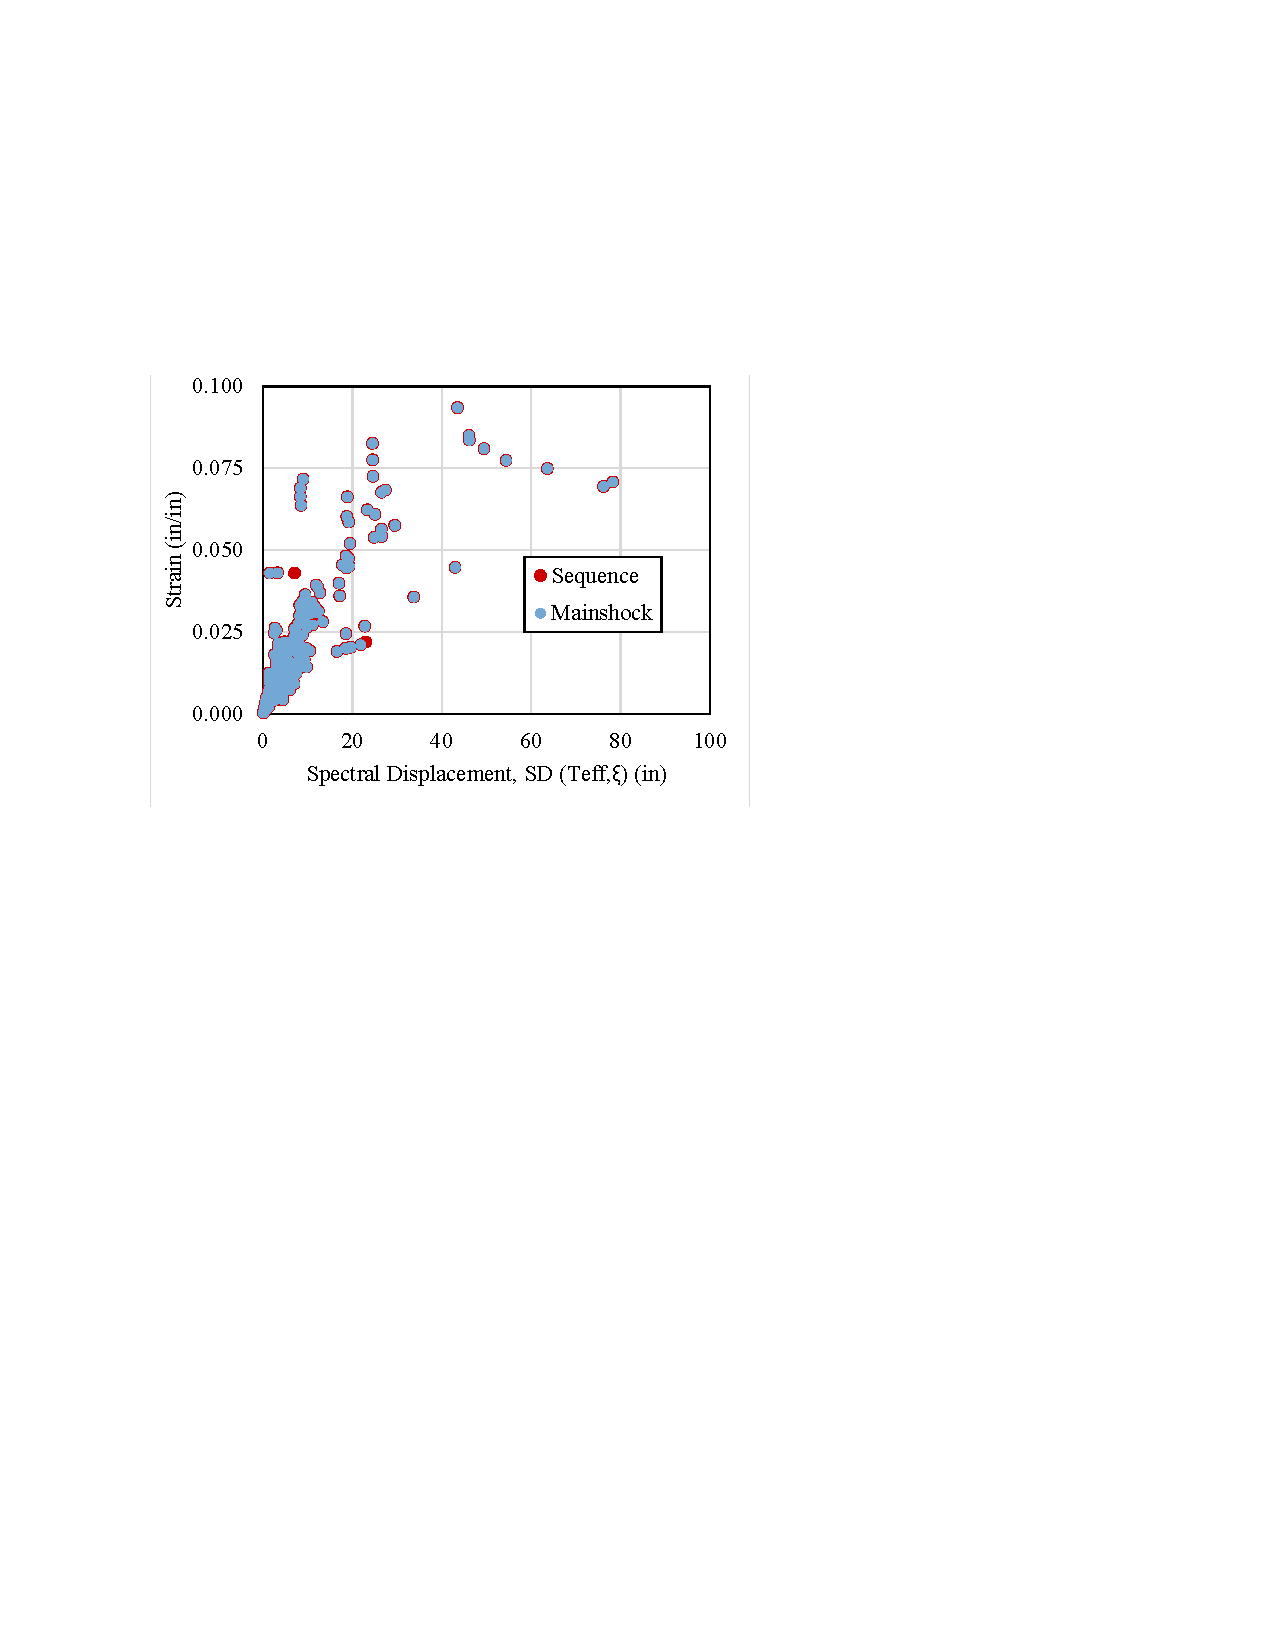
\includegraphics[width=0.65\textwidth]{VAC Thesis 2.0/Chapter-5/figs/MS_AS_results_noincrease_in_demands.pdf}
	\caption{Non Linear Time History Analysis (NLTHA) results showing no increase in the strain demands due to as recorded mainshock-aftershock sequence}
	\label{fig:ms_as_results}
\end{figure}

\subsection{Effect of corrosion level on Strain demands $(\varepsilon)$}

The strain demands $(\varepsilon)$ were plotted against the spectral displacement at the effective period and the equivalent structure damping ($Sd(T_{eff},\xi)$). These two parameters seem to have a linear correlation for all the corrosion levels evaluated. These results are shown in \fref{fig:all_results_nltha}

\begin{figure}[htbp]
	\centering
	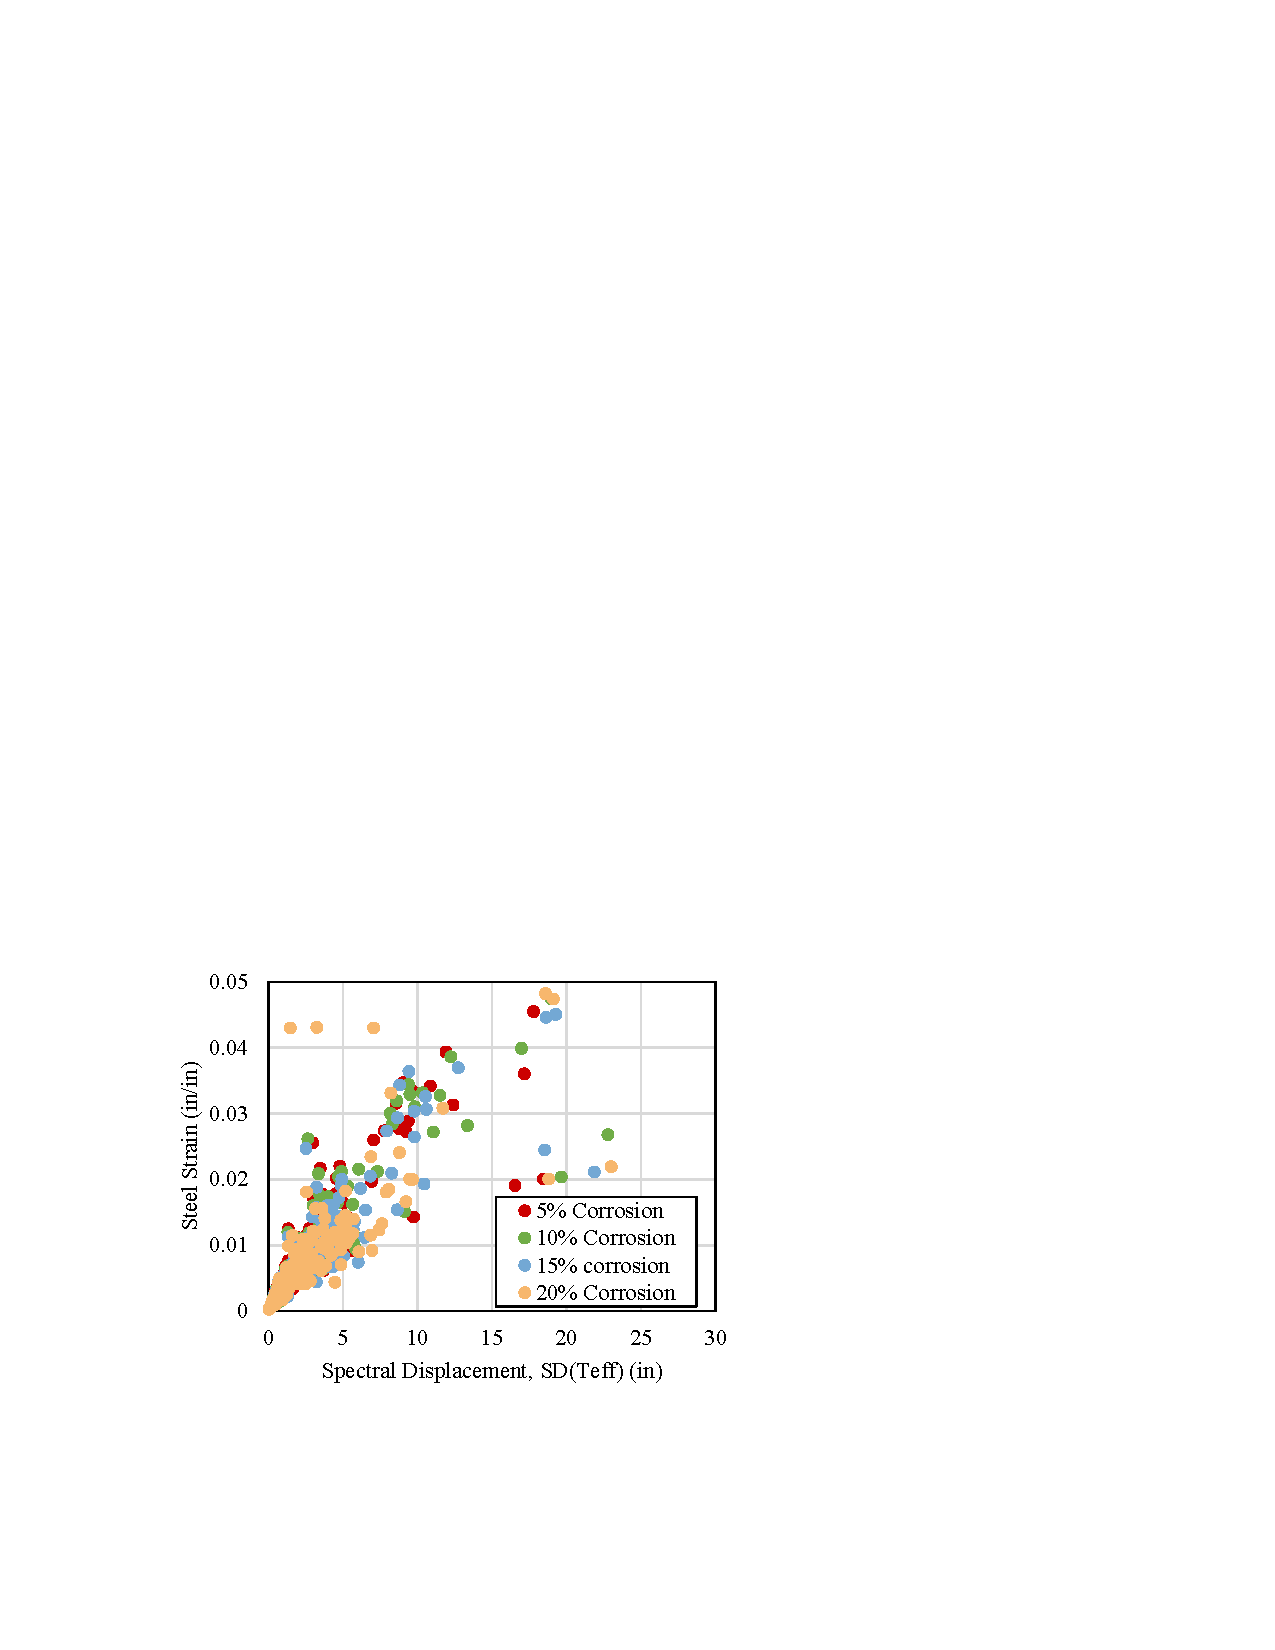
\includegraphics[width=0.65\textwidth]{VAC Thesis 2.0/Chapter-5/figs/All_results_NLTHA_Figure.pdf}
	\caption{Non Linear Time History Analysis (NLTHA) results for Strain demands vs Spectral Displacement at Effective Period $(T_{eff})$, and Equivalent Damping $(\xi)$}
	\label{fig:all_results_nltha}
\end{figure}

The multi-stripe analysis(MSA) was used to obtain a series of cumulative distribution functions to evaluate the effect of corrosion and other variables. The most impactful variables are the corrosion level and the axial load ratio. The effect of these variables are shown in \fref{fig:CDF_strain_vs_ALR}. These figures show that as corrosion level increases, the mean spectral displacement required to preclude a given limit state is decreased. Similarly, the effect of the axial load ratio becomes substantial as it increases.

\begin{figure}[htbp]
	\centering
	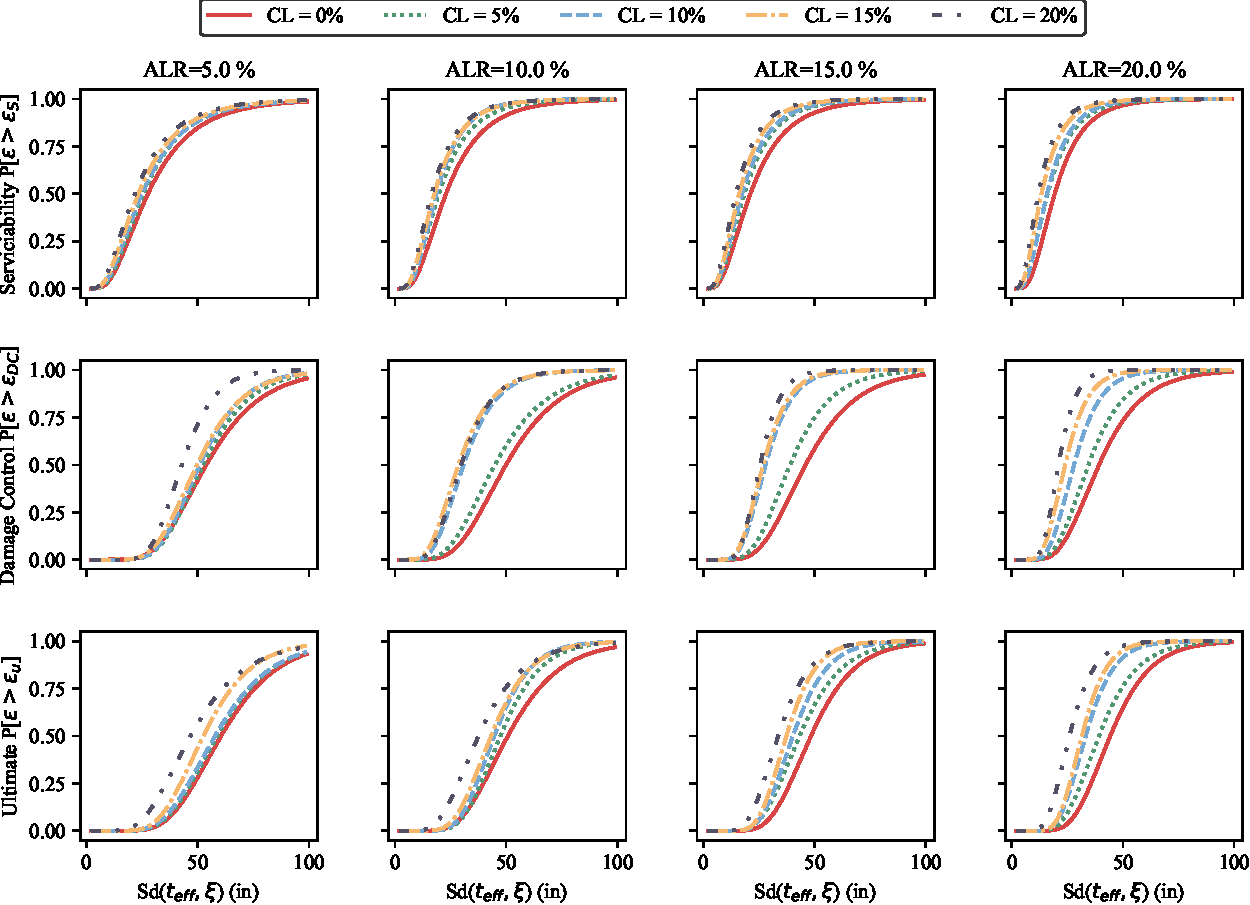
\includegraphics[width=0.9\textwidth]{VAC Thesis 2.0/Chapter-5/figs/CDF_summary.pdf}
	\caption{Cumulative Distribution Function (CDF) for steel strain limit states and different Axial Load Ratios (ALR)}
	\label{fig:CDF_strain_vs_ALR}
\end{figure}

In order to observe the effect of corrosion level and axial load ratio, the mean spectral displacement, defined ad the point where the probability of reaching a limit state is 50\% ($P(\varepsilon>\varepsilon_{ls}=0.5$), is plotted against these two variables. The results are shown in \fref{fig:mean_prob_vs_CL}.

From the results shown in \fref{fig:mean_prob_vs_CL}, two main tendencies can be observed. First, as corrosion level increases, the mean spectral displacement required to reach a limit state decreases, thus precluding an earlier limit state in a corroded structure. It also appears that there is a significant drop at a corrosion level of 10\% ($CL=10\%$), especially for the damage control limit state and the ultimate limit state. This result indicates that a corrosion level this high has potentially undesirable consequences. Research performed on RC members has shown that corrosion levels of 10\% are brittle. Thus, these results are congruent with those observations.

The second observation is that Axial Load Ratios (ALR) greater of 10\% and higher have a more significant drop in their performance due to corrosion. This ALR value is commonly found in bridges, thus the importance of limiting the corrosion level that bridge columns develop in their service years.

\begin{figure}[htbp]
	\centering
	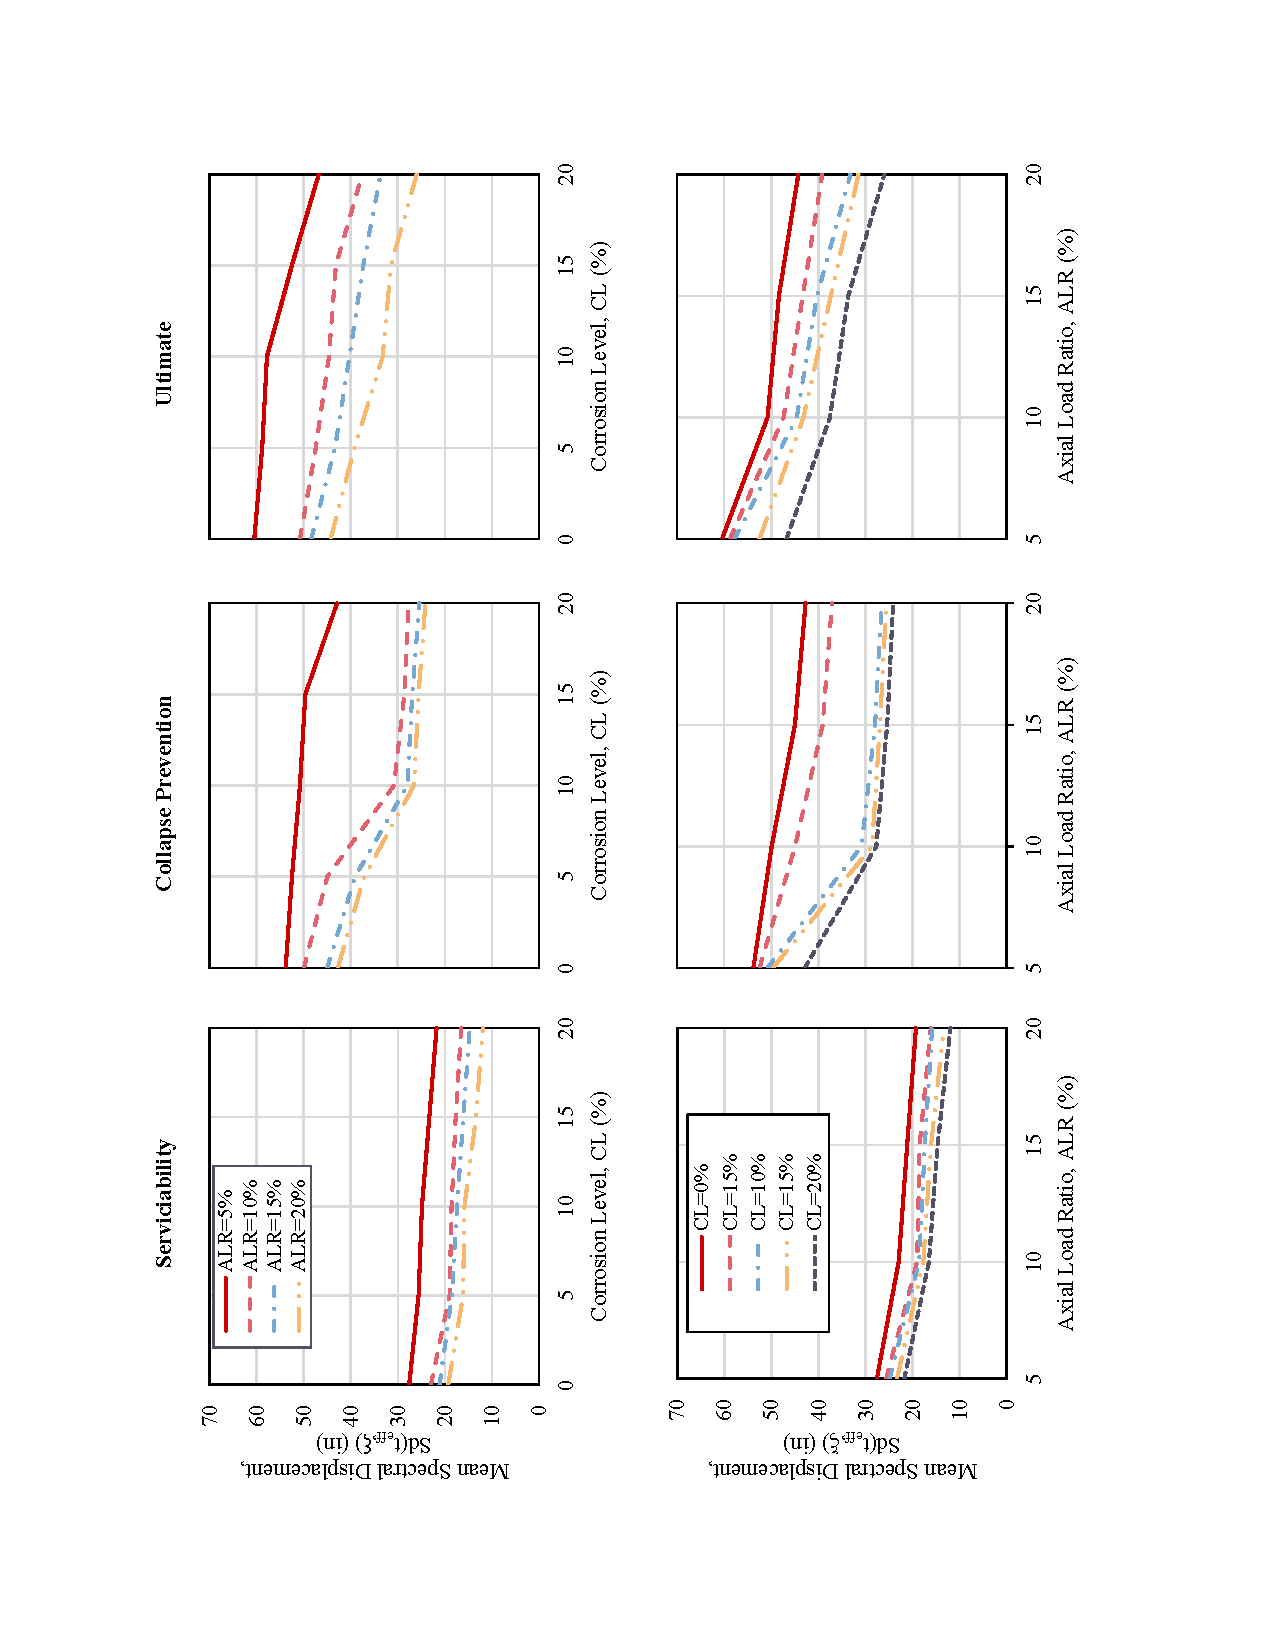
\includegraphics[width=0.85\textwidth]{VAC Thesis 2.0/Chapter-5/figs/Analysis_of_Mean_SDs.pdf}
	\caption{Analysis of mean values $(P=0.5)$ for performance limit states}
	\label{fig:mean_prob_vs_CL}
\end{figure}

The results obtained from these analyses are essential since they provide limiting values for the level of corrosion that could be acceptable in new structures and assessment of existing structures. Therefore, a limiting value for the level of corrosion in new designs should be between 0\%-5\%. For existing structures, a maximum acceptable level of corrosion could be set at $CL=10\%$. This recommendation is made because existing structures would not have been designed to account for aging or corrosion inhibitors. These existing structures would have to consider the effective properties and reduce the cross-section of the reinforcing steel bars. 

Further studies on limit states of corroded structures while improving the outcomes here identify and improve the design and assessment of RC members.

\subsection{Discussion of results}

The Nonlinear Time History Analysis results show that, in general, there is an increase in the strain demands due to corrosion. The increase in the strain demands depends on the limit state being evaluated and the axial load ratio. 

For all limit states, a corrosion level of 10 percent is a reasonable estimate of the maximum acceptable corrosion level. This result agrees with observed behavior in large-scale tests conducted on RC members. An ideal maximum level of corrosion is a 5\% corrosion level.

A limitation of this study was the use of limit state equations based on pristine condition elements with modern detailing. While the limit state equations provide the overall effect of corrosion in RC structures, future studies will provide more information on limit states for aged structures with and without modern detailing.

Therefore, the analytical program agrees with observed experimental material tests conducted as part of this research and observations on corroded RC member tests. Thus, for the design of new structures, it is recommended that an acceptable level of corrosion range is 5\%-10\%. Moreover, for assessment, it is recommended that if a corrosion level greater than 10\% is found, an NLTHA must be performed to assess the existing structure. This analysis will have to consider the effective mechanical properties of the reinforcing steel and the reduction in the cross-sectional properties. These recommendations are applied in the following chapter. 

Another interesting finding was that the effect as recorded sequences of mainshock-aftershock appears negligible. This result is in agreement with previous studies performed on MDOF systems that included degradation of the system in steel frames \cite{Ruiz-Garcia2011}. However, other studies that rely on altered records obtain the opposite result because they change the frequency content of their records.